\chapter{NVM Based Write-behind Caching} \label{chapt: checkpointing}
HPC applications process large amounts of data that have to be written (read) to (from) large shared files residing in the global parallel file system. In order to make the dataset manageable, 
this is usually partitioned into smaller subsets and assigned to available cores for parallel processing. Complex datasets such as multi-dimensional arrays are logically flattened into a linear 
sequence of bytes and striped across several I/O targets for best performance. This results into the loss of the original spatial locality. Due to this characteristic, accesses to spatially contiguous 
regions translate into non-contiguous accesses to the file. Therefore, applications generating a large number of small, non-contiguous I/O requests to the parallel file system usually experience 
degradation of I/O performance. Such performance degradation is known as the small I/O problem and is related to the fact that parallel file systems provide best I/O bandwidth performance for large 
contiguous requests, while they typically provide only a fraction of the maximum available bandwidth in the opposite case~\cite{ChingCLP06}~\cite{HeSSYT11}. This is due to the large number of RPCs 
generated by the file system clients overwhelming I/O servers, the resulting high number of hard disk head movements in every I/O target (seek overhead) and, ultimately, to the restrictions imposed 
by the POSIX-IO write semantics that generates lock contention on file systems' blocks.

Having recognised the small I/O problem, collective I/O was proposed by the MPI-IO community~\cite{ThakurGL99}. Collective I/O exploits global I/O knowledge in parallel I/O to a shared file. This 
knowledge is used to build an aggregated view of the accessed region in the file and coalesce all the corresponding small non-contiguous requests into a smaller number of large contiguous accesses, 
later issued to the parallel file system. 

In this chapter we present our approach to improve collective I/O performance using non-volatile memory devices in HPC clusters' compute nodes. The fundamental observation that motivates our approach 
is that collective I/O performance is limited by the slowest aggregator. Aggregators experience different run-times mainly for two reasons: the communication pattern required to build file domains might 
differ among aggregators and the scheduling of requests in I/O servers might not happen simultaneously for all aggregators. These two factors, in conjunction with the need for global synchronization 
between following rounds of two phase I/O, represent the main cause of suboptimal performance.

The motivation for using a file system based write-behind approach in collective I/O is that at Exascale the amount of memory per core will shrink~\cite{ASCAC2010}. For this reason we need to make 
sure that main memory is dedicated to progressing in the computational tasks instead of the caching of large out-of-core arrays. Non-volatile memory devices provide an additional memory tier right 
between the DRAM and HDDs and can thus be used effectively as fast persistent buffers to mask remote file access time.

The remainder of this chapter is organized as follow: in Section~\ref{sec: ext2ph} we describe in detail the extended two phase algorithm at the base of the collective I/O implementation in ROMIO;
in Section~\ref{sec: coll_io_limit} we review the main performance bottlenecks in the extended two phase algorithm providing, whenever available, possible solutions to overcome each of them; 
in Section~\ref{sec: nvm-approach} we discuss in detail our proposed solution to address global synchronization limitations; finally, in Section~\ref{sec: nvm-related} we review the related works 
and outline the main differences with our approach.

\section{Extended Two Phase Algorithm} \label{sec: ext2ph}
We now describe in detail the ext2ph algorithm implementation in the ROMIO middleware. We pin-point where the major contributions to performance are located and on what aspect of collective I/O they
reflect. Figure~\ref{figure: coll_io_impl} shows the ext2ph algorithm flow diagram for collective write operations in aggregators; the diagram for non-aggregators is similar but does not contain write 
functions. (Collective read operations are not described since the behaviour is specular to the write case.) The diagram divides the algorithm into three main phases: an initialization phase (on the 
extreme left end side), the shuffle phase (on the extreme right end side), and the write phase (in the center).

\begin{figure}[H]
  \centering
  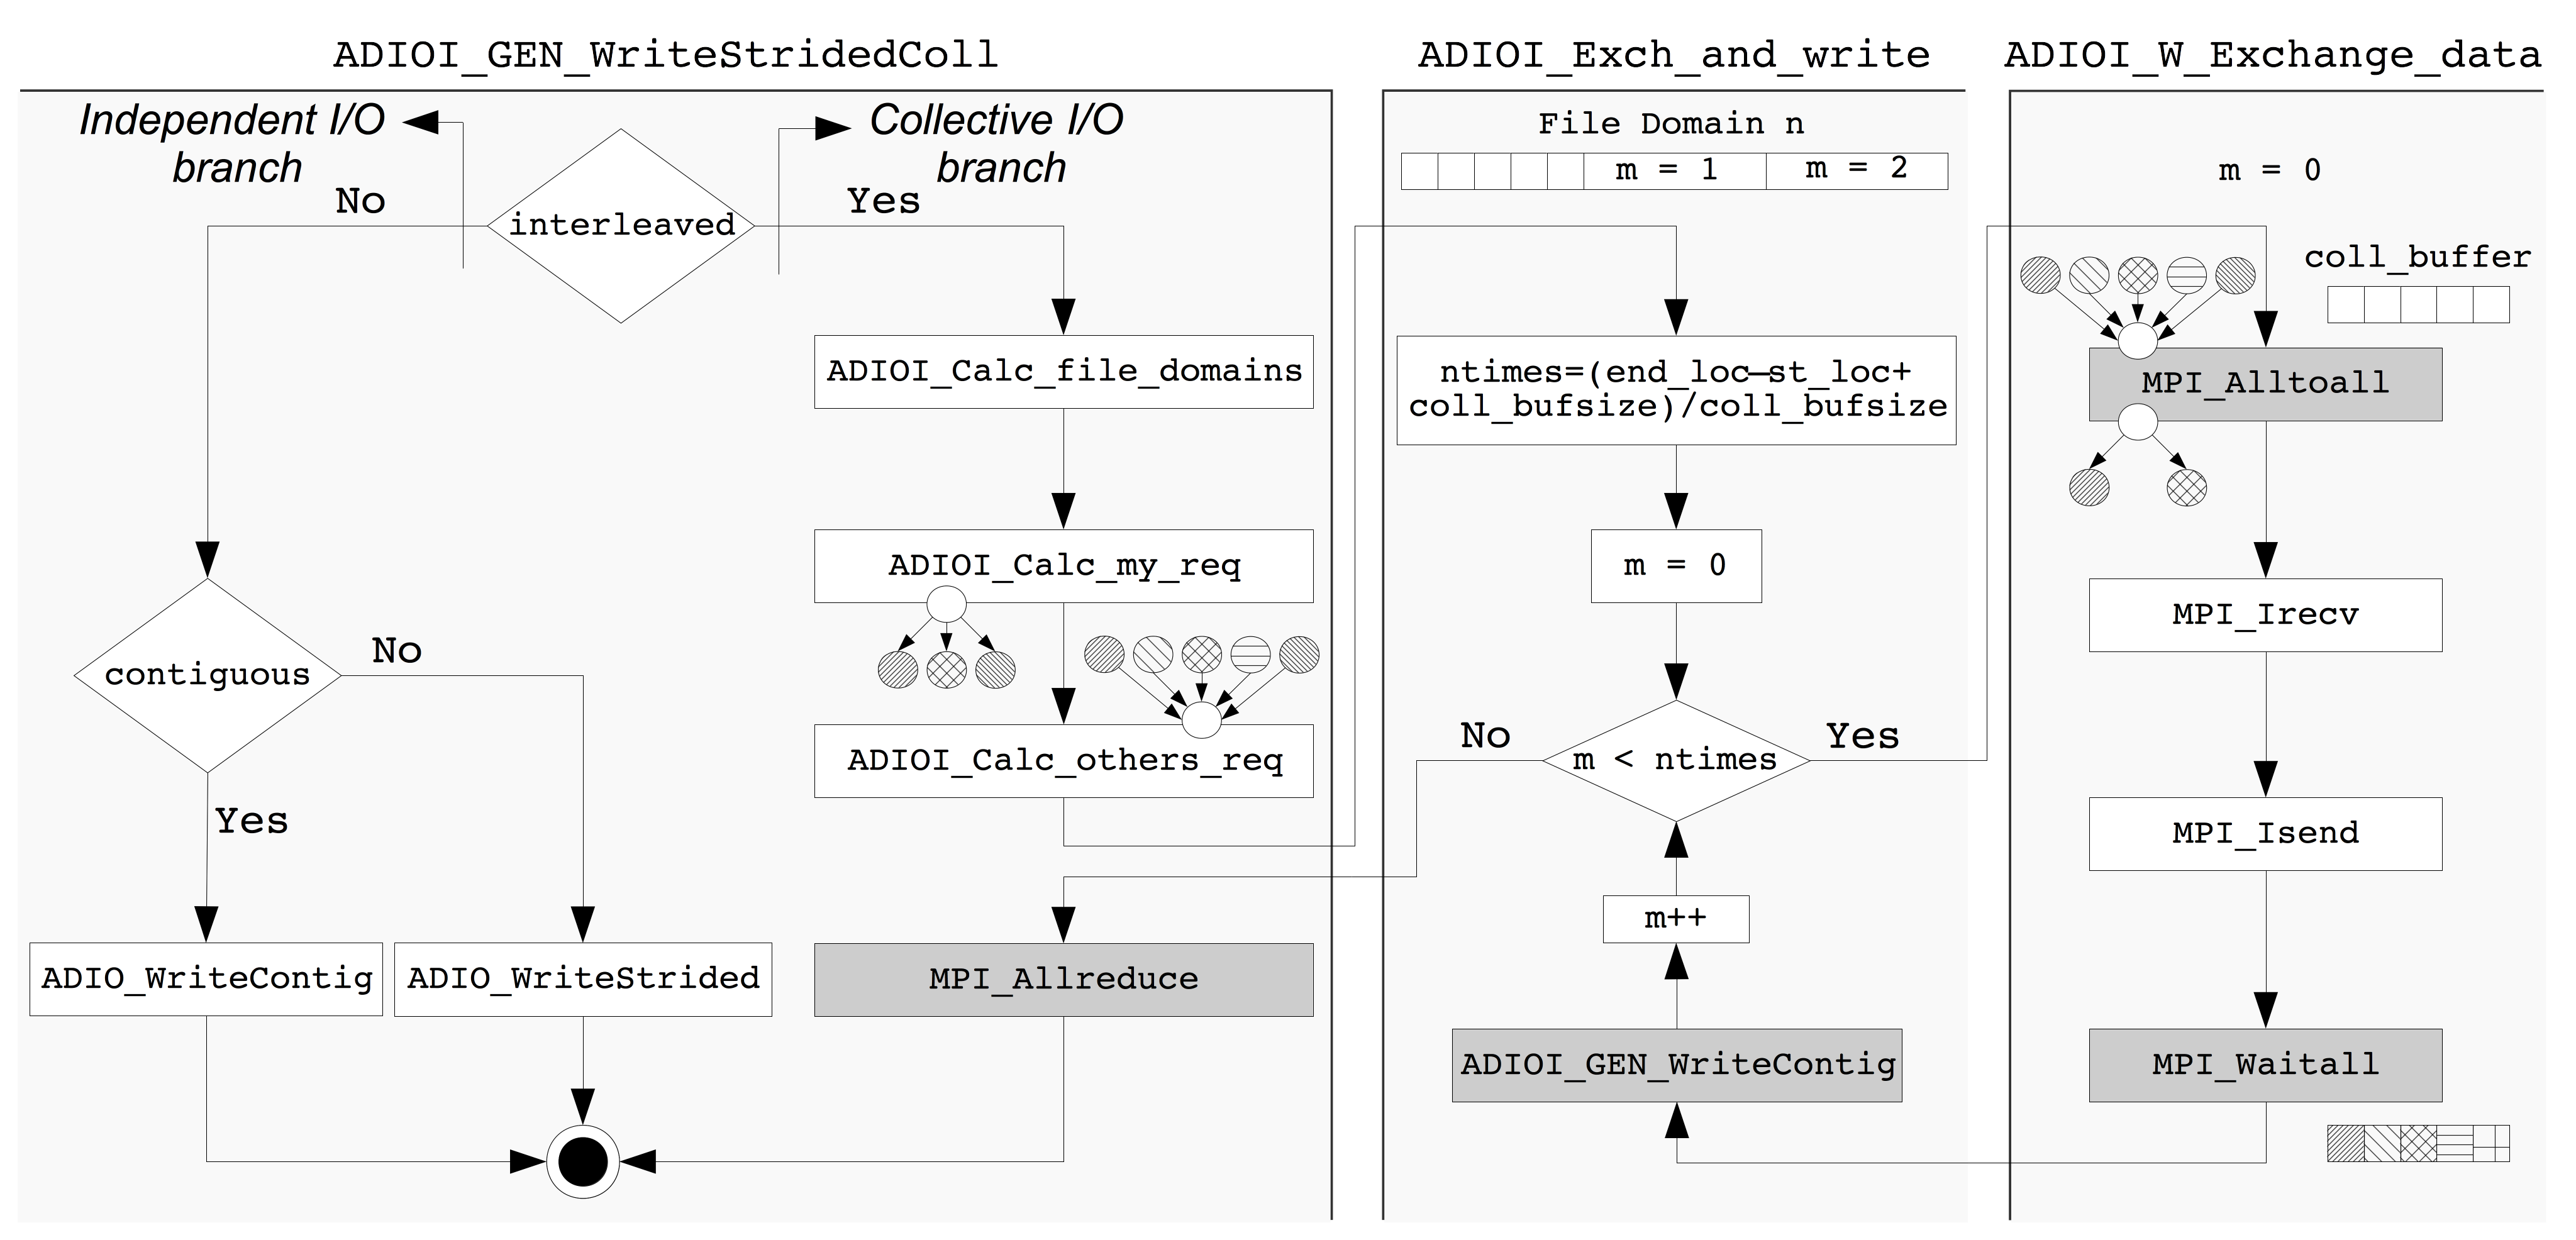
\includegraphics[angle=90, width=0.8\textwidth]{figures/ext2ph_t}
  \caption{Collective I/O flow diagram for the write path in aggregators (non-aggregators neither receive nor write any data, just send it to aggregators). \codeword{MPI\_File\_write\_all()} 
  invokes \codeword{ADIOI\_GEN\_WriteStridedColl()}. Performance critical functions for the collective I/O branch are highlighted in grey.}
  \label{figure: coll_io_impl}
\end{figure}

The \texttt{MPI\_File\_write\_all()} and \texttt{MPI\_File\_write\_at\_all()} functions are translated into the \texttt{ADIOI\_GEN\_WriteStridedColl()}\footnote{ADIOI\_LUSTRE\_WriteStridedColl() for Lustre.} 
function in the presented diagram. This function is responsible for the initialization of the ext2ph algorithm. First, it computes the file domains by dividing the aggregated access region by the number of 
available aggregators (\texttt{ADIOI\_Calc\_file\_domains}) as shown in Equation~\ref{formula: aggr-region}.

\begin{equation}\label{formula: aggr-region}
    \ceil*{\frac{MAX(end\_offset) - MIN(st\_offset)}{cb\_nodes}}
\end{equation}

Second, for every process it computes to what file domain requests belong (\texttt{ADIOI\_calc\_my\_req}) and third, for every aggregator it keeps track of what other requests fit into the file domain handled 
by the aggregator. The tracking information is stored into a \textit{file domain access table} (FDAT) and each aggregator has one to remember what parts of the file domain belong to which process in the 
application. FDATs are implemented using two arrays, one for the starting offsets and one for the lengths\footnote{A process might have more than one request for the same file domain.}. The FDATs arrays
have an entry for every process in the application, even if the process has no data in that file domain.

Once the initialization phase is complete, two phase I/O can start. Because file domains might not fit entirely in main memory, they can be broken down into smaller units using a collective buffer 
(by default this is only a few MB in size) and two phase I/O is carried out in multiple rounds of data shuffling and I/O. The central part of the diagram contains a \textit{for} loop that is iterated 
once for every round of two phase I/O. The number of rounds is computed dividing the file domain by the collective buffer size (\texttt{coll\_bufsize}).

At the beginning of the data shuffling phase (on the right end side of the diagram) every process has to communicate to aggregators what part of their file domain will be exchanged in that round. This is 
done using the \texttt{MPI\_Alltoall()} collective communication function. Afterwards, every aggregator invokes a non-blocking receive operation (\texttt{MPI\_Irecv()}) and can optionally send its own data
to other aggregators by invoking a non-blocking send operation (\texttt{MPI\_Isend()}). Finally, every aggregator waits for all the send and receive to complete by invoking \texttt{MPI\_Waitall()}. 

When the shuffling phase has completed, the collective buffer contains all the required data and it can be written to the file using \texttt{ADIOI\_GEN\_WriteContig()}. This function internally calls the standard 
POSIX-IO write operation. When all the file domains have been written to the file, aggregators need to exchange error codes to make sure that each of them has completed correctly and user buffers can be reused
for another collective write operation. This task is performed by invoking \texttt{MPI\_Allreduce()}.

There are three main performance contributions to the ext2ph implementation just described: (\textbf{a}) global synchronisation cost; (\textbf{b}) communication cost; and (\textbf{c}) write cost. \codeword{MPI\_Allreduce()} 
and \codeword{MPI\_Alltoall()} account for global synchronisation cost; when a process reaches them it has to wait for all the other processes to arrive before continuing. Because aggregators are the
only processes writing data to the parallel file system, they experience the highest run-time and the slowest aggregator among all governs the overall collective I/O performance. \codeword{MPI\_Waitall()} 
accounts for communication cost since every process first issues all the non-blocking receives (if any) and sends, and afterwards waits for them to complete. Finally, \codeword{ADIOI\_GEN\_WriteContig()} 
accounts for write cost.

The collective I/O behaviour in ROMIO can be controlled by users through a set of MPI-IO hints. Users can decide whether collective I/O should be enabled or disabled with \codeword{romio\_cb\_write} and
\codeword{romio\_cb\_read} (for write and read operations respectively), how many aggregators should be used during a collective I/O operation with \codeword{cb\_nodes} and how big the collective 
buffer should be with \codeword{cb\_buffer\_size}. Table~\ref{table: coll_io_hints_table} summarises the hints just described.

\begin{table}[!htb]
\centering
\ra{1.5}
\caption{Collective I/O hints in ROMIO.}
\newcolumntype{K}{>{\centering\arraybackslash} m{3cm}}
\newcolumntype{V}{>{\centering\arraybackslash} m{5.5cm}}
\begin{tabular}{KV}
\toprule
\bf \small Hint & \bf \small Description \\
\midrule
\small \codeword{romio\_cb\_write} & \small \codeword{enable} or \codeword{disable} collective writes \\
\small \codeword{romio\_cb\_read} & \small \codeword{enable} or \codeword{disable} collective reads \\
\small \codeword{cb\_buffer\_size} & \small set the collective buffer size [bytes]\\
\small \codeword{cb\_nodes} & \small set the number of aggregator processes\\
\bottomrule
\end{tabular}
\label{table: coll_io_hints_table}
\end{table}

Each of these hints has an effect on collective I/O performance. For example, by increasing the number of aggregators there will be a higher number of nodes writing to the parallel file 
system and thus a higher chance that one of these will experience variable performance due to different scheduling time at I/O servers, with increasing write time variation and associated 
global synchronisation cost. Furthermore, by increasing the collective buffer size users can reduce the number of two phase I/O rounds and, consequently, the number of global synchronisation 
events. Bigger collective buffers also affect the write cost since more I/O servers will be accessed in parallel potentially increasing the aggregated I/O bandwidth.

Besides the hints described in Table~\ref{table: coll_io_hints_table}, there are other hints that do not directly concern collective I/O but affect its performance. The first is the 
\codeword{striping\_factor} hint, which defines how many I/O targets (servers) will be used to store the file. The second is the \codeword{striping\_unit} hint, which defines how big the data chunks 
written to each I/O target will be (in bytes). These two hints change the file characteristics in the parallel file system and typically the striping unit also defines the block size and thus the locking 
granularity for the file (e.g., Lustre).

\section{Collective I/O Limitations} \label{sec: coll_io_limit}
%In Chapter~\ref{chapt: background} we have described in detail the extended two phase algorithm at the base of the collective I/O implementation in ROMIO. We recall that 
The goal of the extended two phase algorithm is to produce an intermediate I/O pattern in which the aggregated access region, in the logical file representation, is divided into multiple contiguous ranges, 
named \textit{file domains}, that are transfered concurrently and in liaison by aggregators to the file system. Additional interprocess communication is traded against reduced I/O cost, since this typically 
dominates performance. In this section we discuss the limitations in the ext2ph algorithm and provide for each of them possible solutions that have been explored in previous research works.

\subsection{File System Stripe Contention}
POSIX compliant file systems use locking to enforce data consistency in the file. Parallel file systems typically adopt an extent based locking strategy in which the client accessing the file
is granted a lock covering a larger portion than requested. Because the process might access other parts of the file in subsequent I/O operations, this strategy reduces the communication between 
the client and the lock manager. The way the extent based locking strategy is implemented differers between file systems. GPFS for example, uses a distributed token based approach in which the 
client requesting access to a region of the file is granted a token covering the whole file. This client becomes the owner of the lock and other clients wishing to access the file have to contact 
it in order to get tokens for other regions of the file. Lustre, on the other hand, uses a centralized server based approach in which a lock for all the file stripes, managed by a specific server,
is granted to the client. The locking mechanisms just described are presented in Figure~\ref{figure: gpfs-lock} and Figure~\ref{figure: lustre-lock} for GPFS and Lustre respectively.

\begin{figure}[!htb]
  \centering
  \begin{subfigure}[t]{0.6\textwidth}
  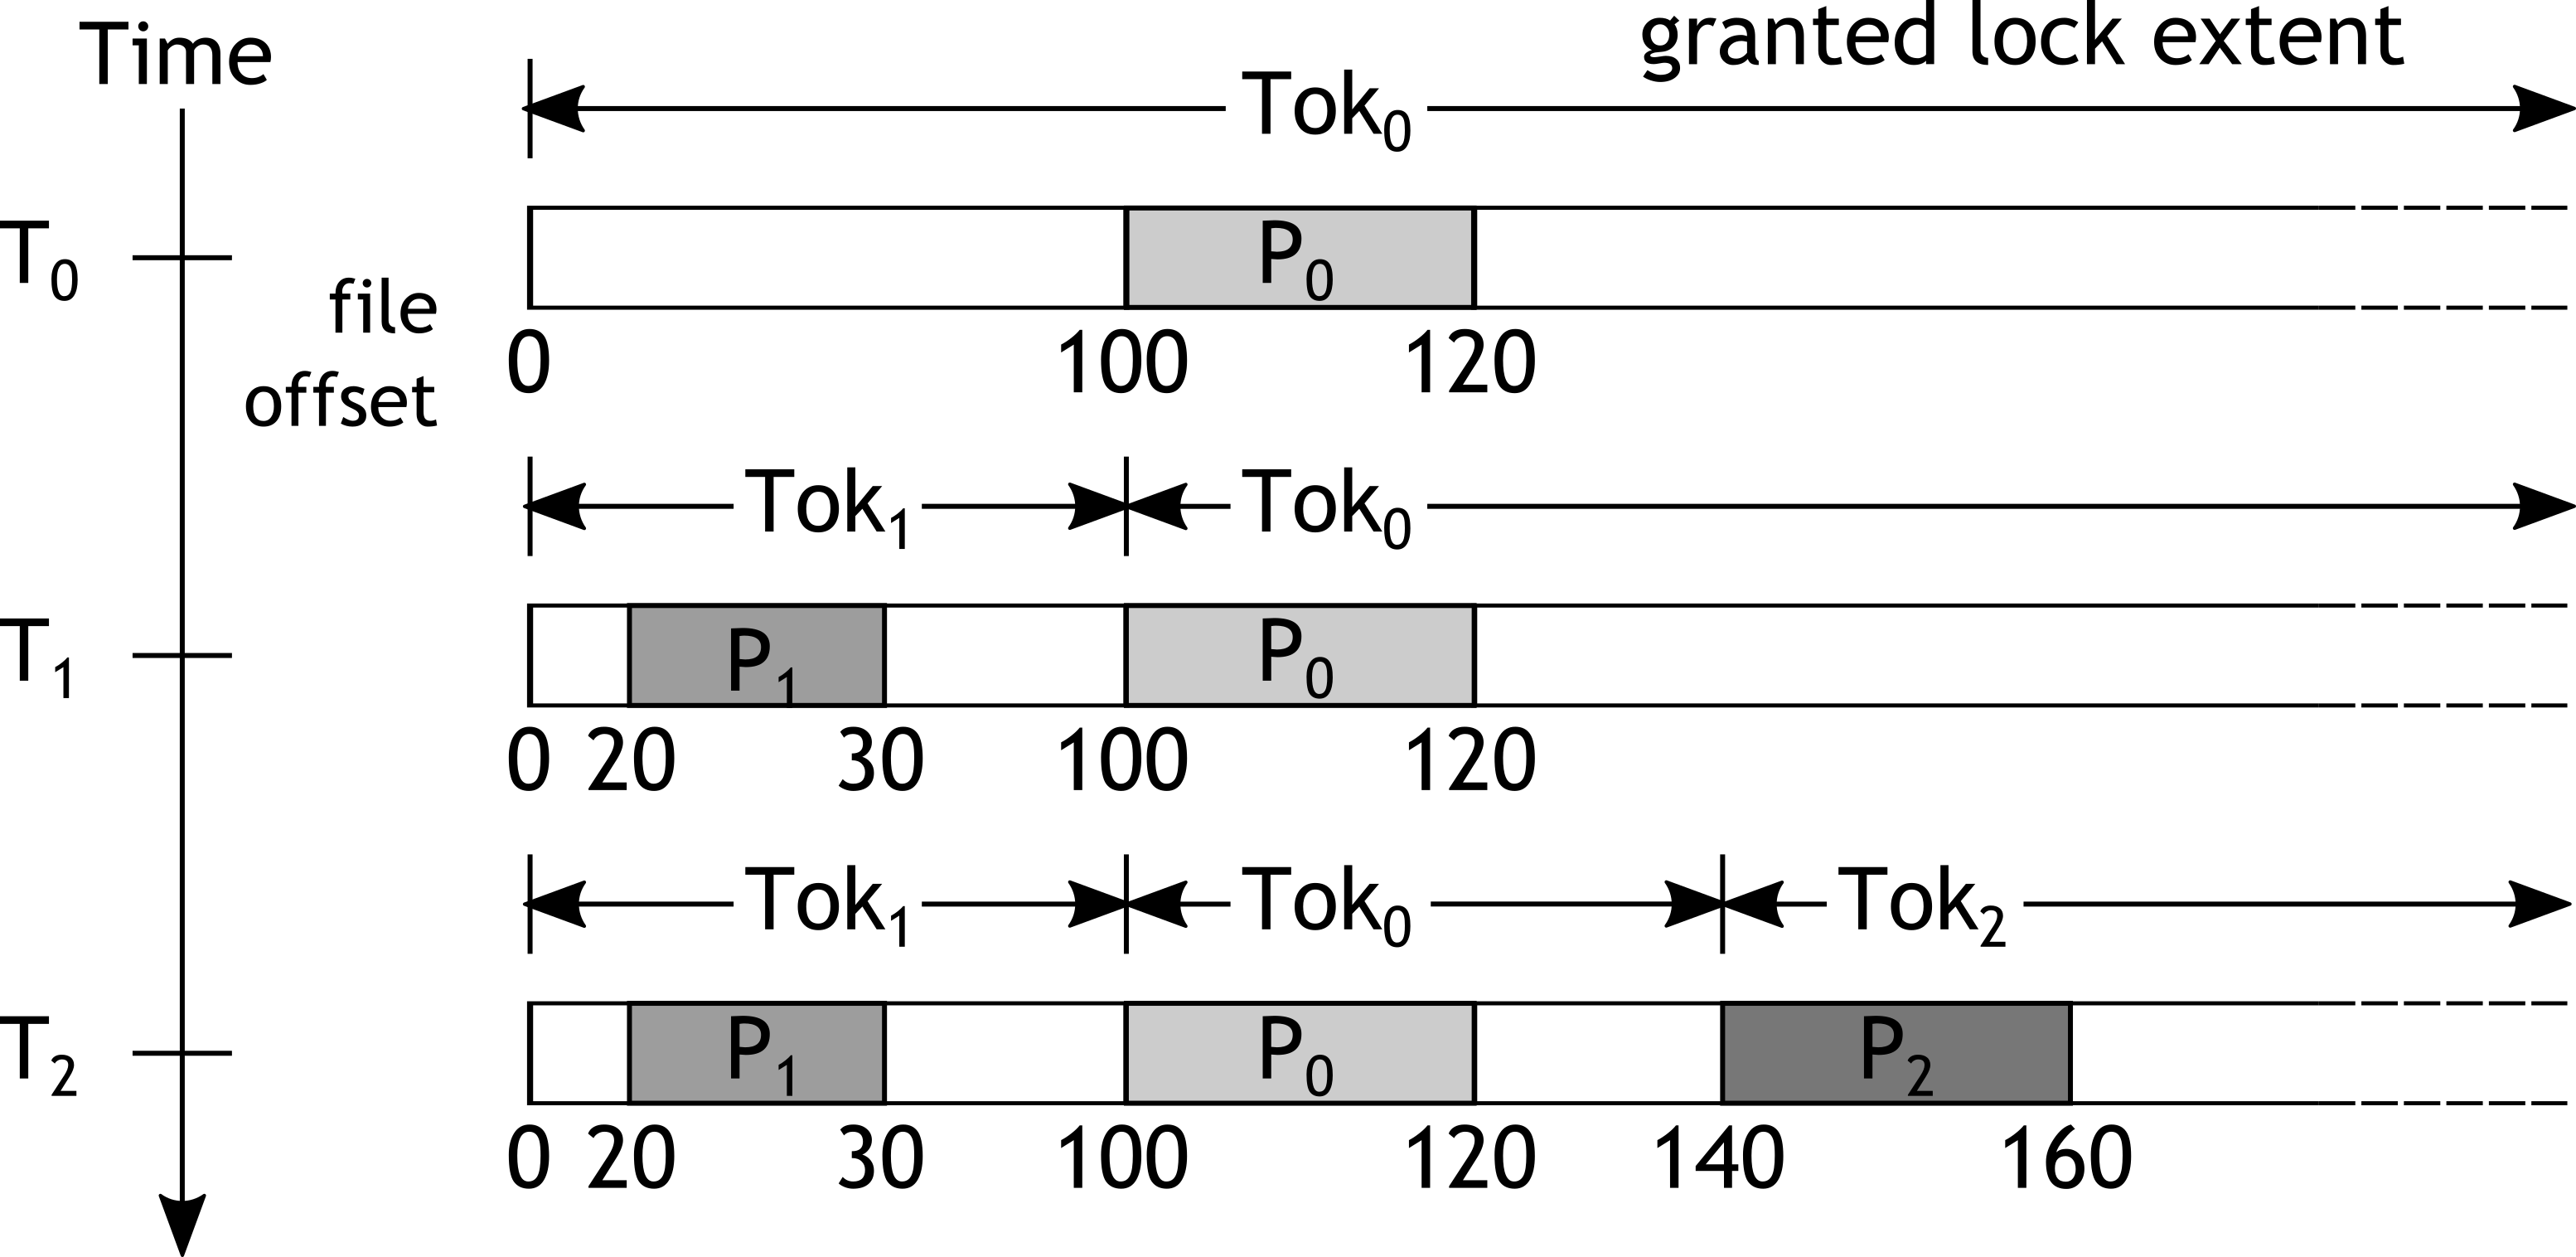
\includegraphics[width=\textwidth]{figures/gpfs-lock}
  \caption{}
  \label{figure: gpfs-lock}
  \end{subfigure}
  \begin{subfigure}[t]{0.6\textwidth}
  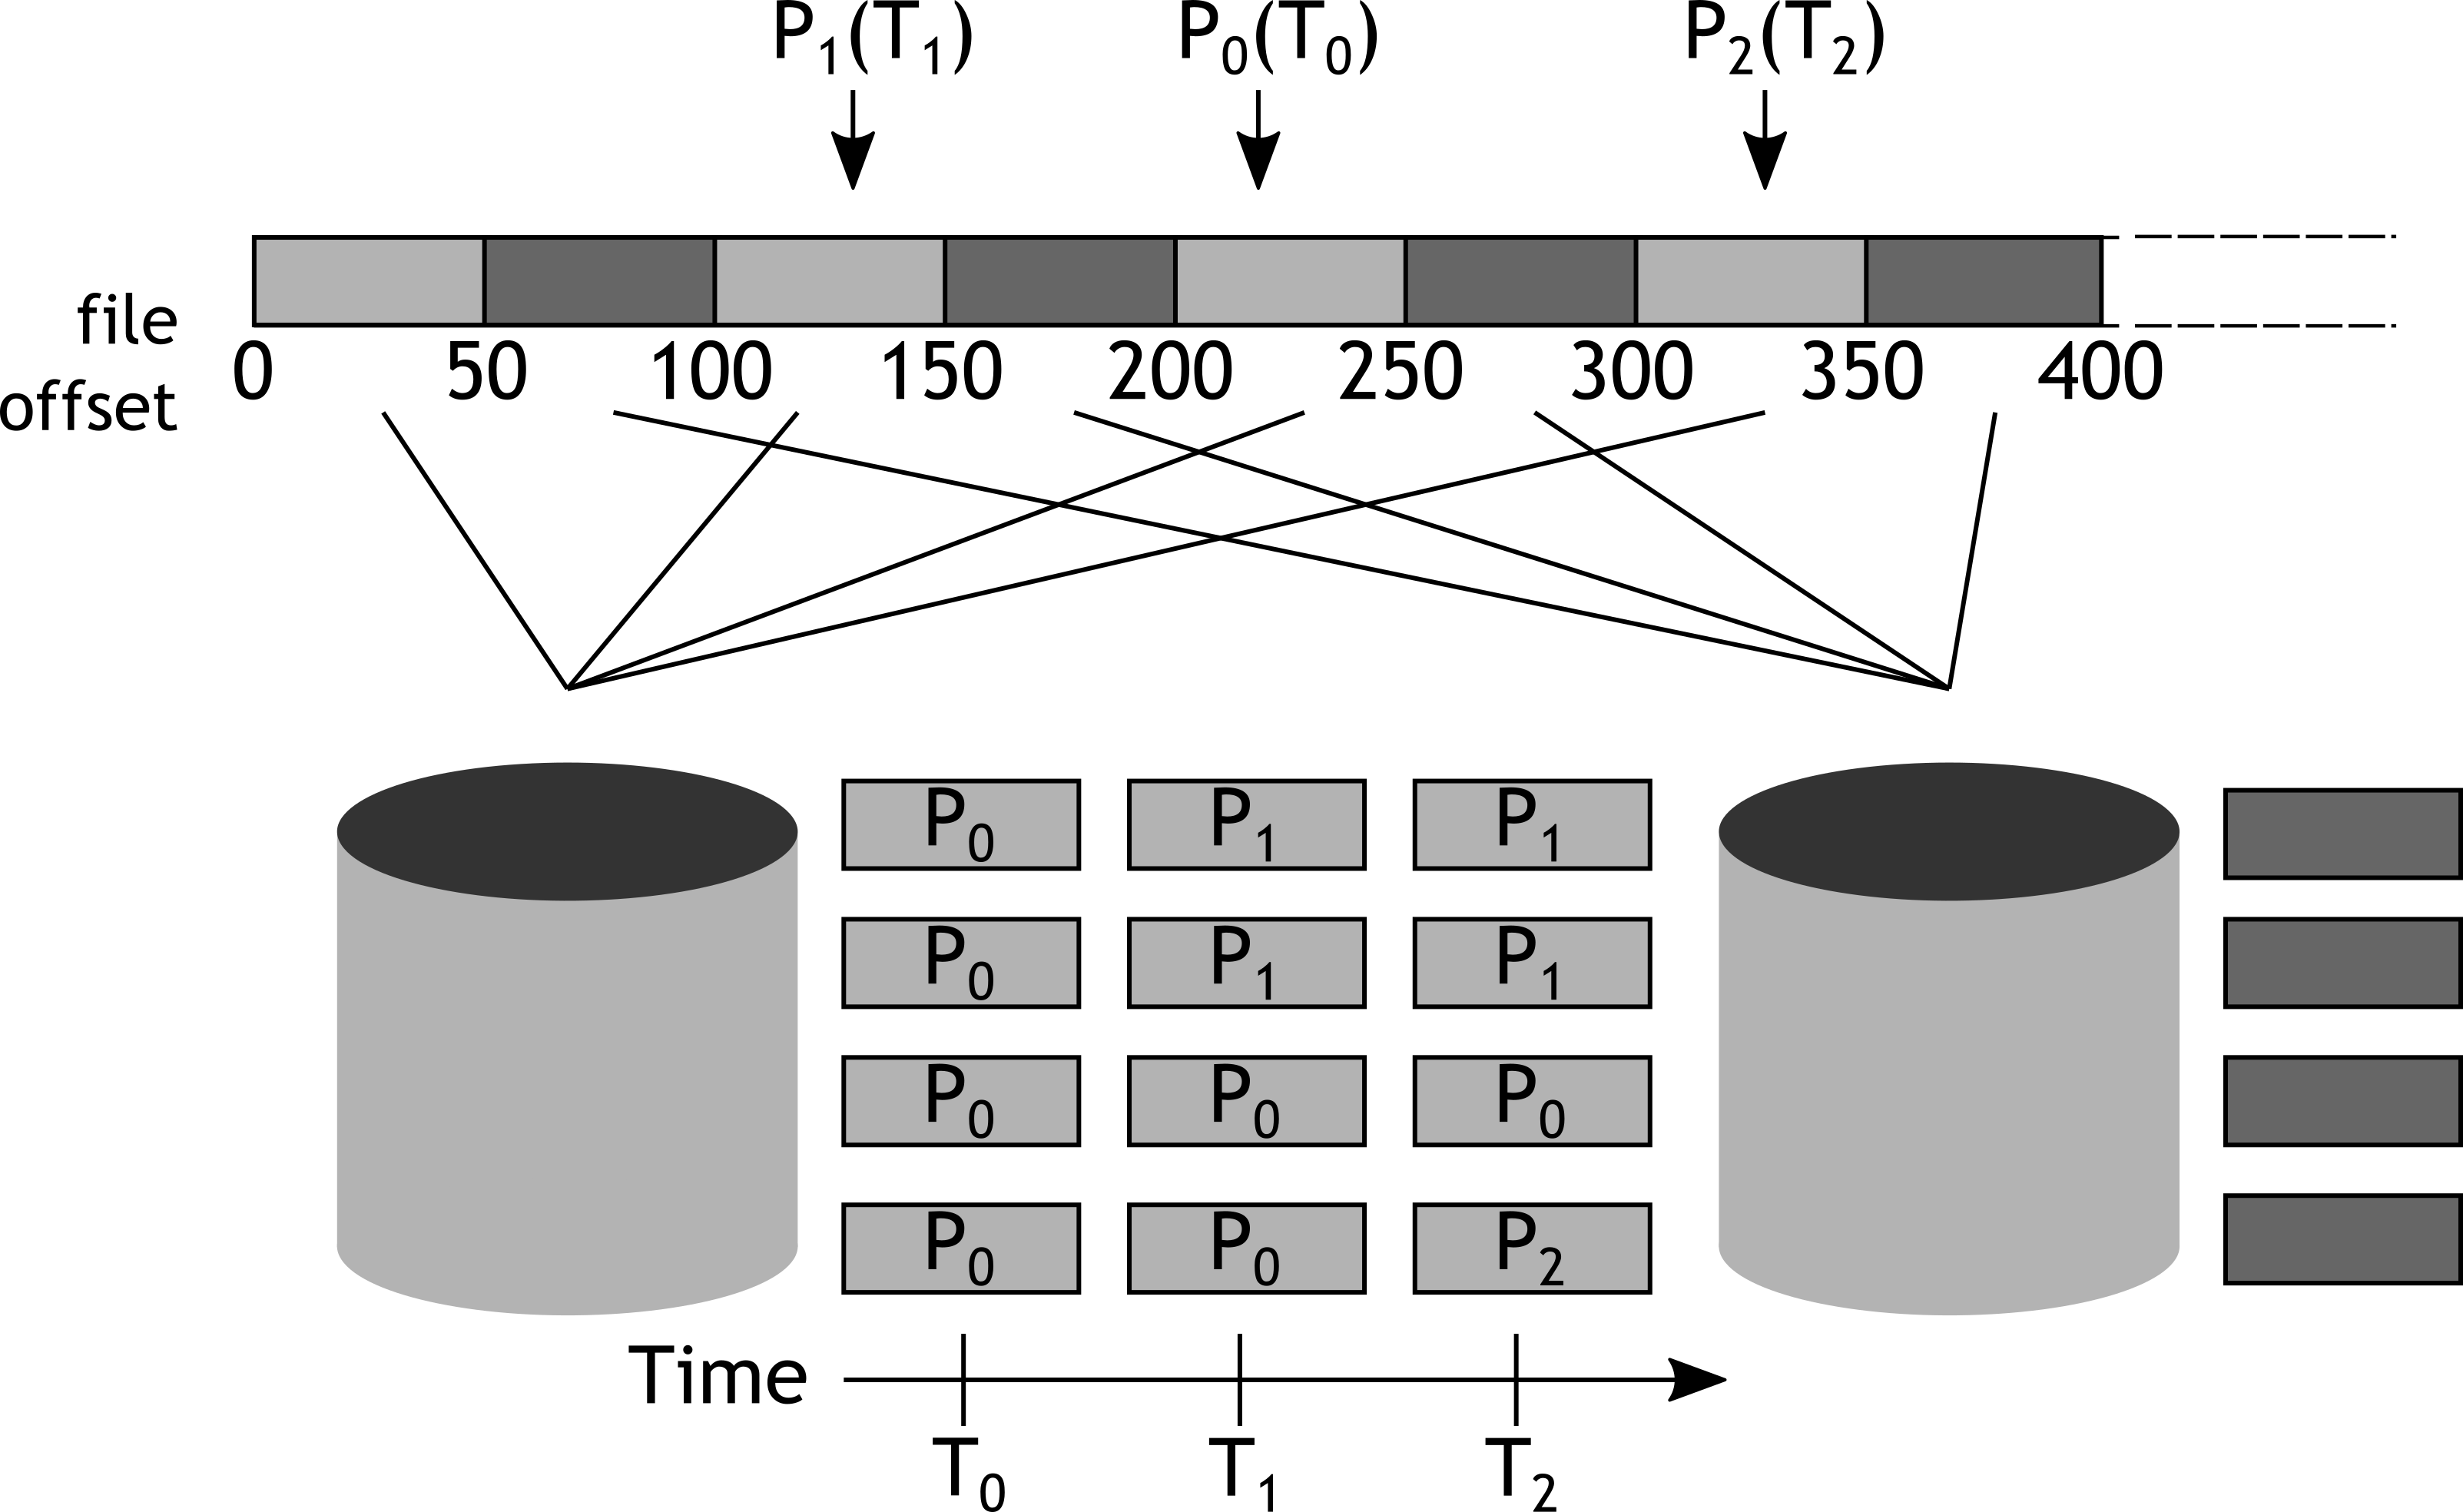
\includegraphics[width=\textwidth]{figures/lustre-lock}
  \caption{}
  \label{figure: lustre-lock}
  \end{subfigure}
  \caption{Extent based locking for GPFS~\ref{figure: gpfs-lock} and Lustre~\ref{figure: lustre-lock}. In both figures there are three process requesting access to different parts of the file
  at different times.}
\end{figure}

In the ext2ph algorithm file domains are built using an even partitioning by default. The even partitioning guarantees an optimal load balancing because every aggregator gets exactly the same
amount of data. Nevertheless, it also allows file systems stripes to be shared among multiple clients, causing false sharing of file system blocks and serializing requests at the file system level.
For this reason, it is important to make sure that file domains are built keeping the file system's locking protocol in mind. A simple solution to the problem of file system stripe contention is to
align file domains to stripe boundaries as shown in Figure~\ref{figure: gpfs-partition}.

\begin{figure}[!htb]
  \centering
  \begin{subfigure}[t]{0.8\textwidth}
  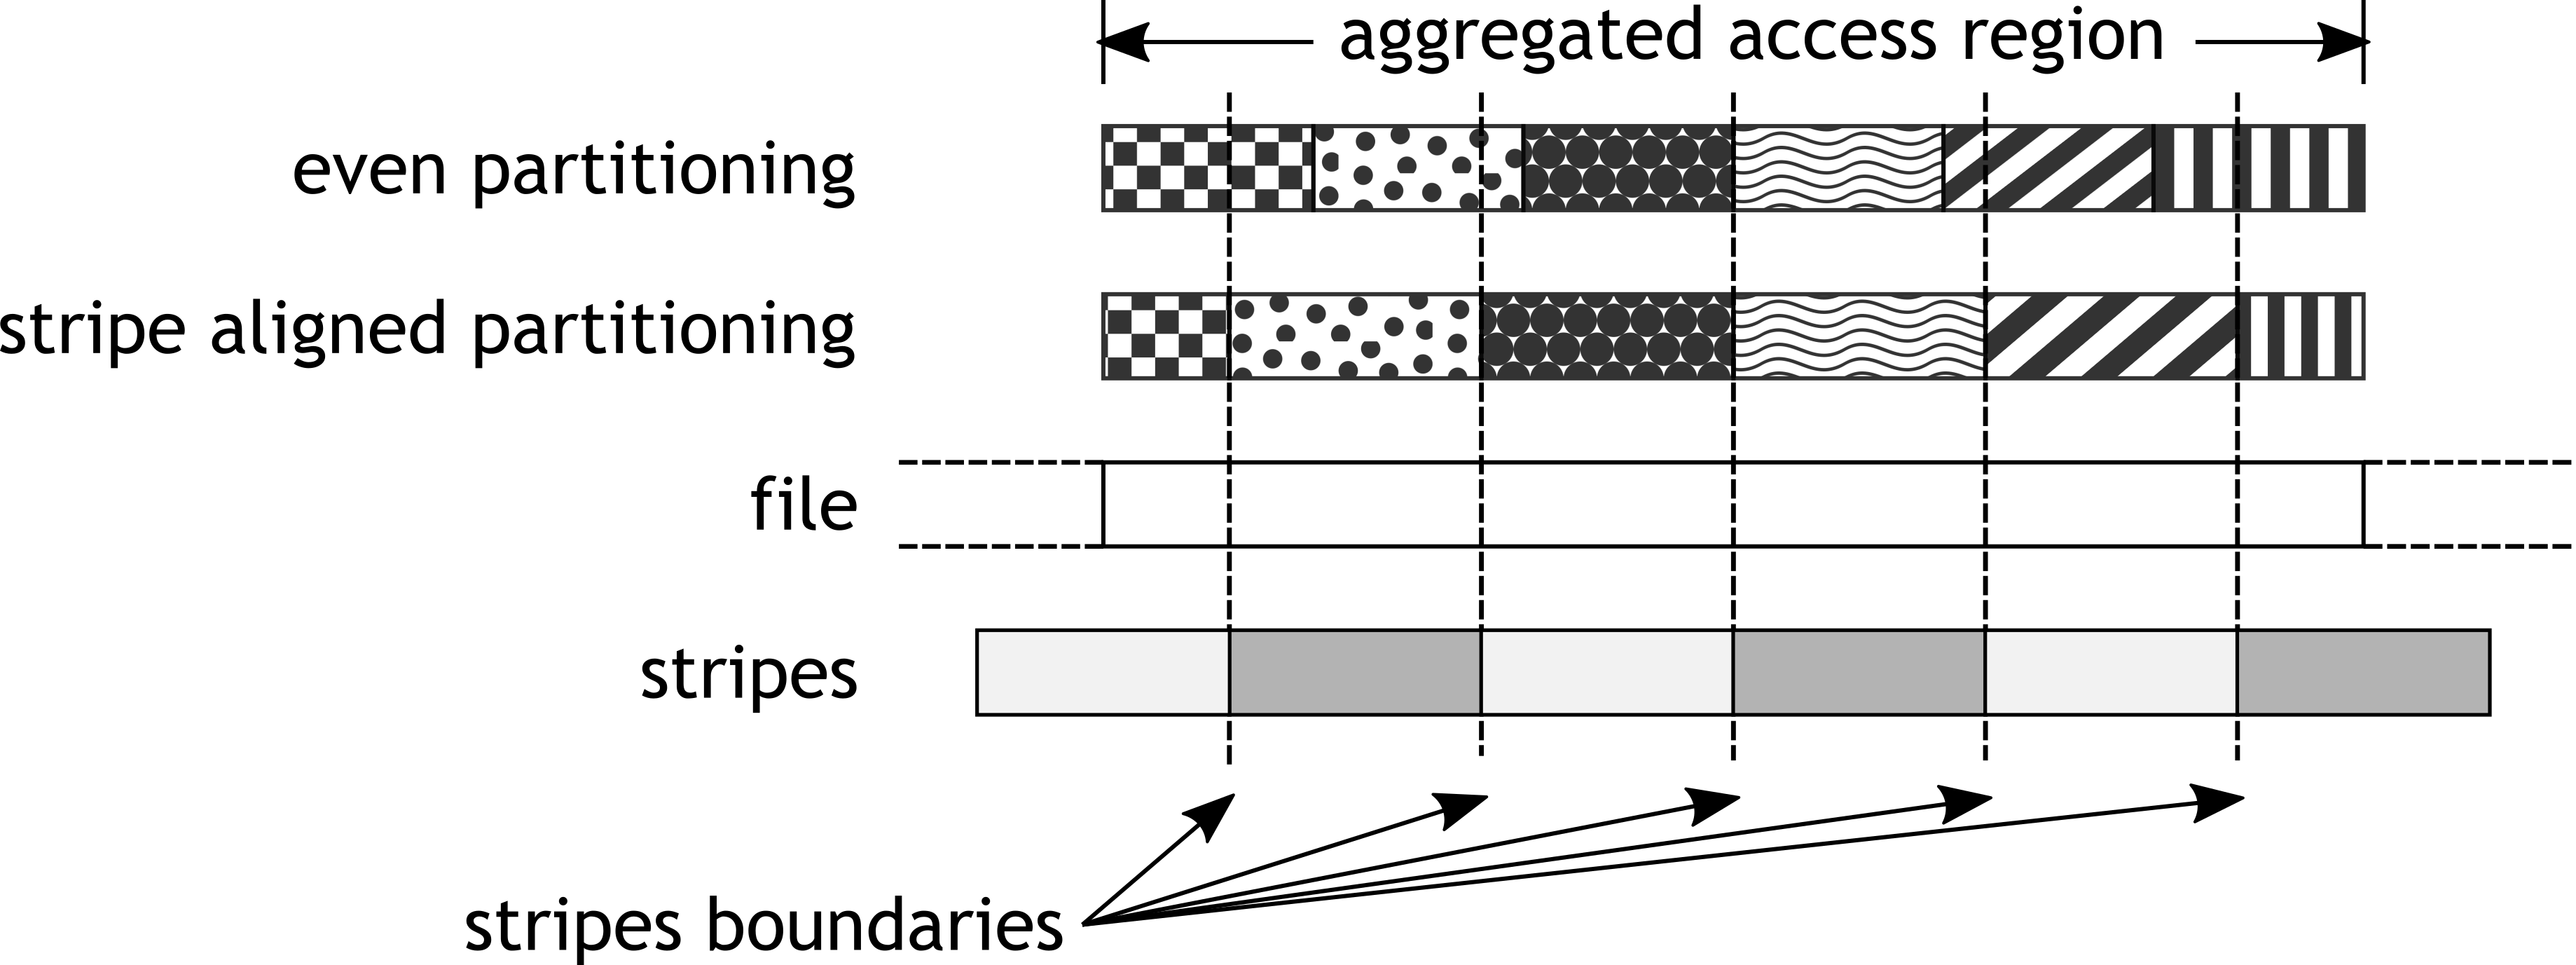
\includegraphics[width=\textwidth]{figures/gpfs-partition}
  \caption{}
  \label{figure: gpfs-partition}
  \end{subfigure}
  \begin{subfigure}[t]{0.9\textwidth}
  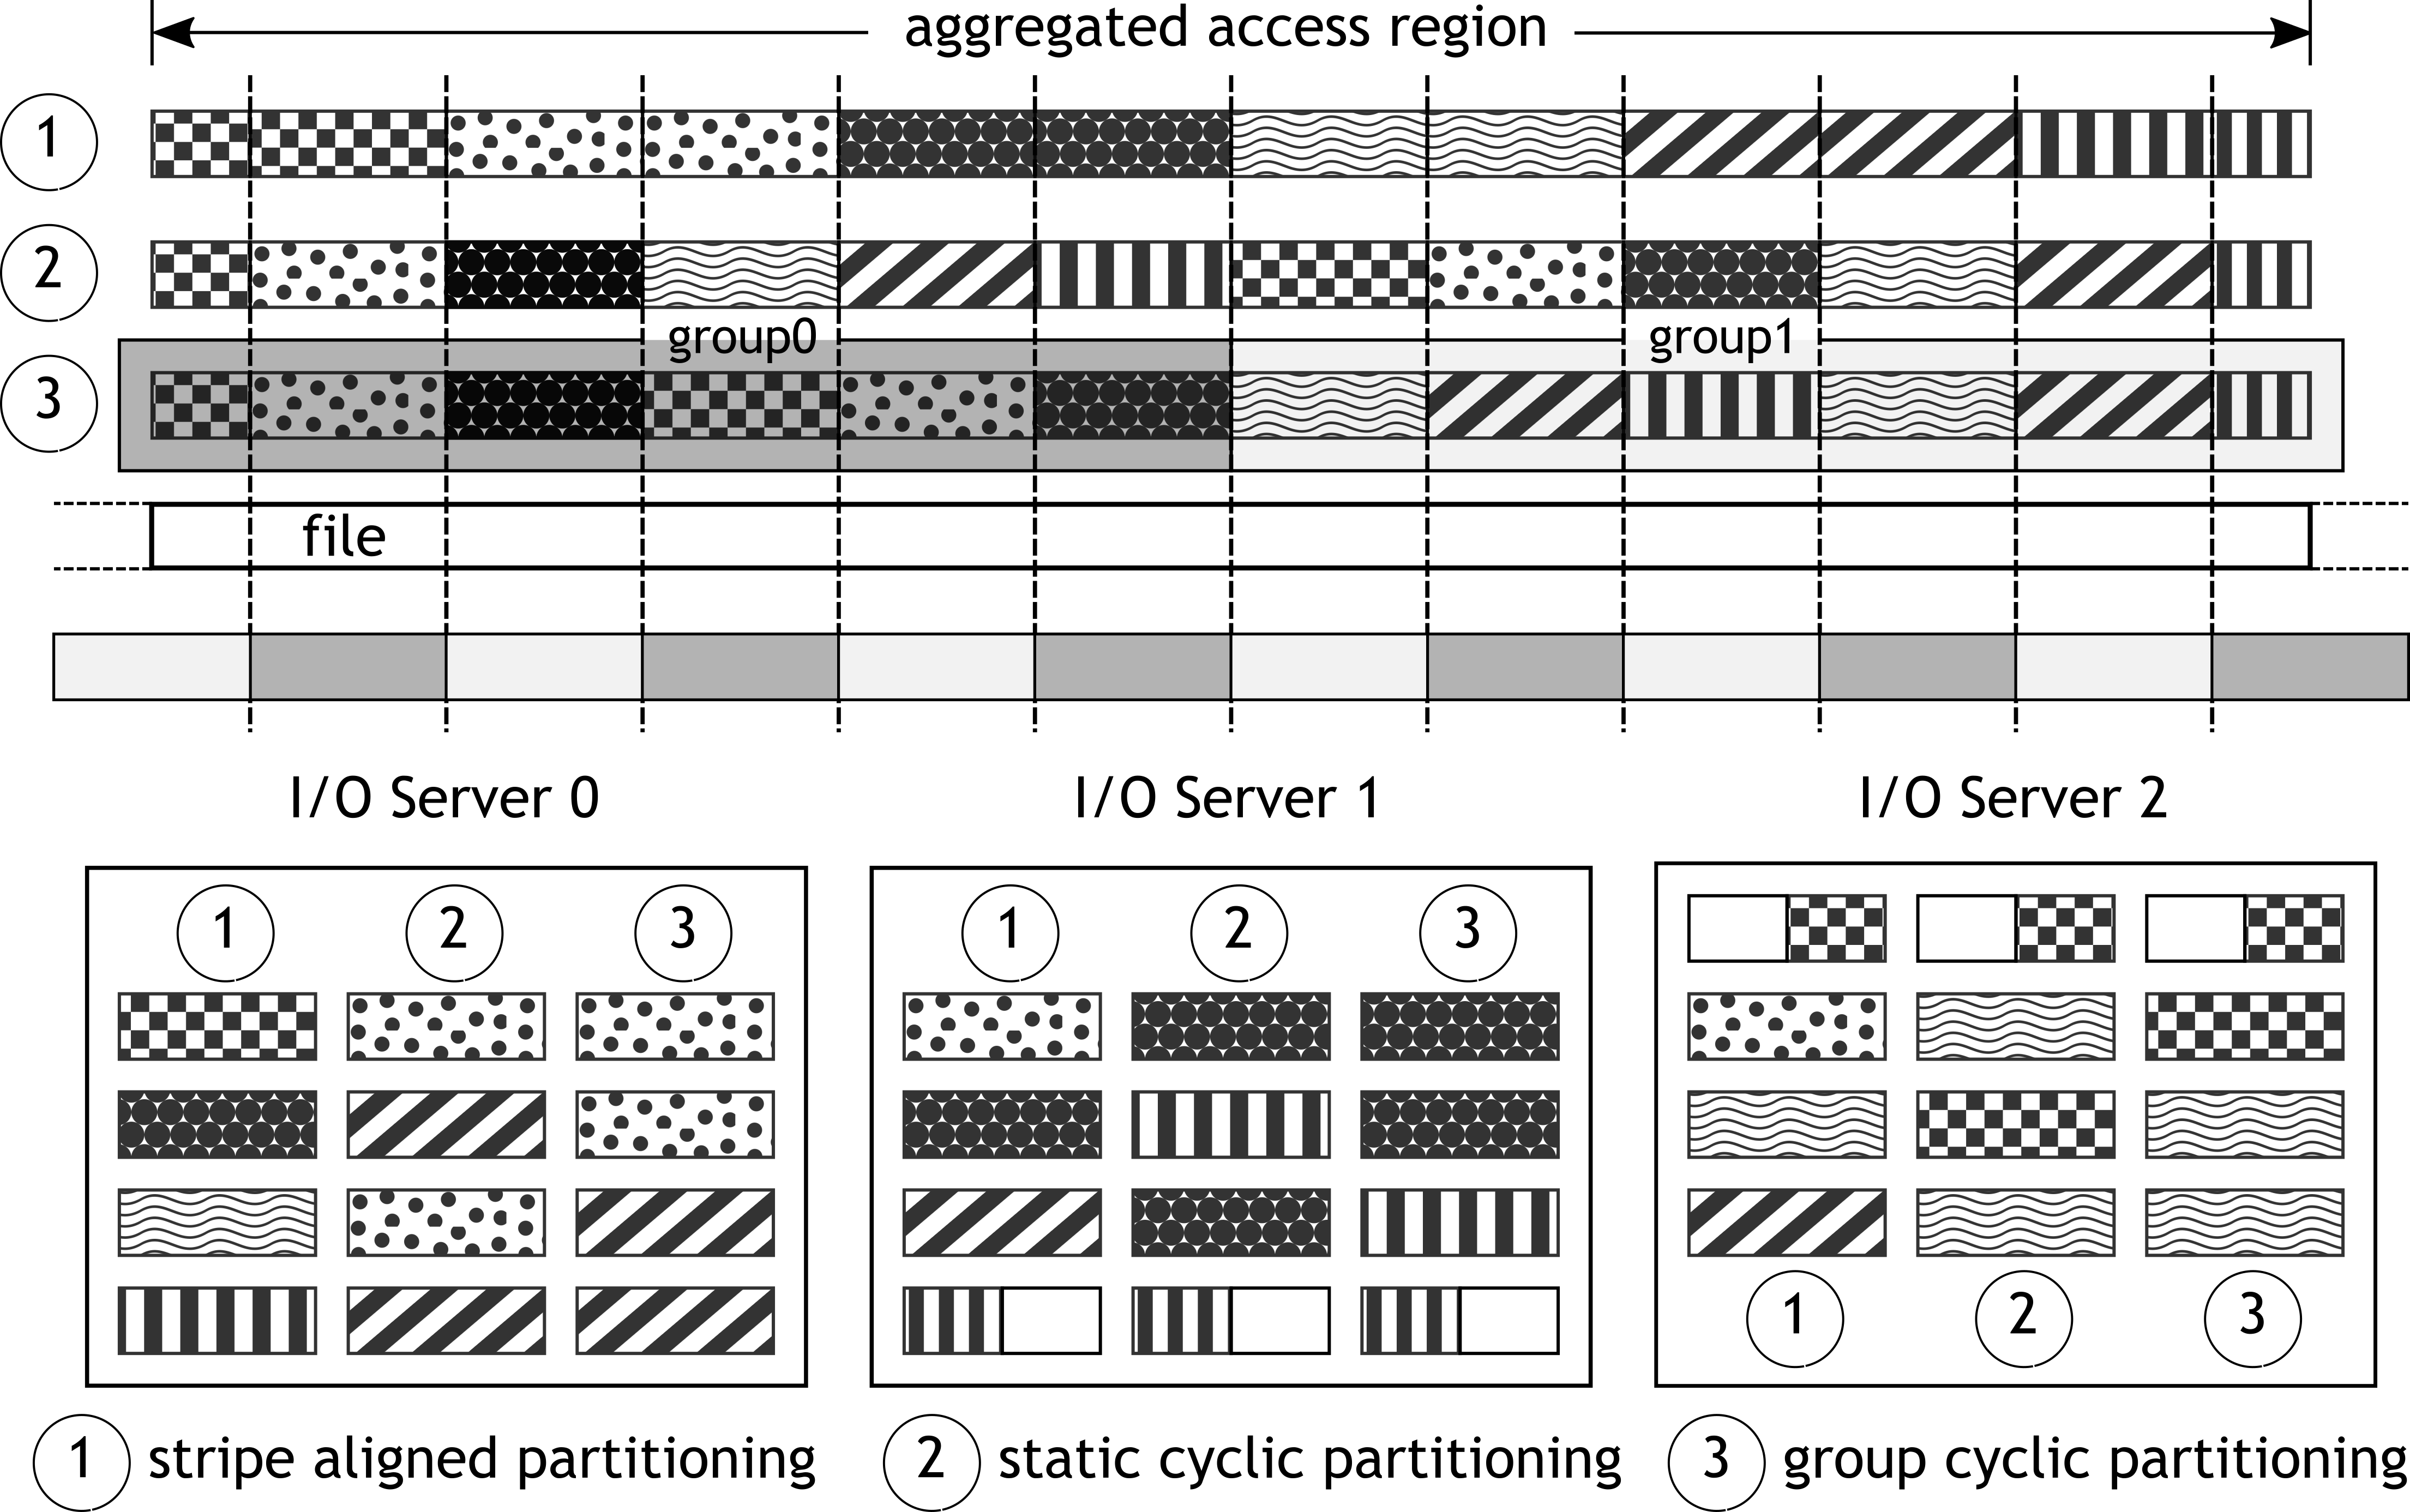
\includegraphics[width=\textwidth]{figures/lustre-partition}
  \caption{}
  \label{figure: lustre-partition}
  \end{subfigure}
  \caption{Possible partitioning strategies for GPFS~\ref{figure: gpfs-partition} and Lustre~\ref{figure: lustre-partition}. File domains, and thus aggregators, are marked with different
  filling patterns.}
\end{figure}

The stripe aligned partitioning works best for GPFS because the token based extent covers the file using the logical offset. For Lustre, on the other hand, the locking protocol depends on how stripes are 
arranged in the I/O servers. Therefore, the stripe aligned strategy causes aggregators to communicate with multiple servers, generating an increased locking protocol overhead. A better partitioning strategy 
would distribute stripes among aggregators in a fixed order, minimizing the communication with multiple servers. This approach is shown in Figure~\ref{figure: lustre-partition} and is called static cyclic 
partitioning. Static cyclic partitioning always assigns stripes to the same aggregator even across multiple I/O operations. This is done by taking the stripe number, dividing it by the number of available 
aggregators and taking the modulo. In this way static cyclic partitioning can also minimize the lock protocol overhead across multiple collective I/O operations. Although static cyclic partitioning can 
reduce locking protocol overhead, it is not yet optimal. To understand why consider case 2 in the figure. In the example, stripes from different aggregators are interleaved in I/O servers. To assign locks 
to each of them the lock manager will need four messages, two for each time the stripes are interleaved. 

A group cyclic partition, as shown in case 3, works better because it arranges stripes belonging to the same aggregator contiguously in the server. In the group cyclic strategy the aggregated access
region is divided into groups, each of these having a number of stripes multiple of the number of I/O servers. Inside each group static cyclic partitioning is then performed to assign stripes to a subset 
of aggregators equal to the number of servers. In the figure, for example, there are three I/O servers and six aggregators. The aggregated access region is therefore divided into two groups. Each group has
six stripes and three aggregators. Using group cyclic partitioning the lock manager only needs two messages to assign the requested locks to the clients.

The interaction between the different file domain partitioning strategies and the locking protocol used by the file system has been studied by Liao and Choudhary~\cite{LiaoA08}~\cite{Liao11}.

\subsection{Logical to Physical Layout Mismatch}
As we have seen in Figure~\ref{figure: lustre-partition} a file in Lustre, as well as in other parallel file systems, is stripped across multiple I/O servers. For this reason the logical file representation
as sequence of blocks does not match the physical layout of data in the parallel file system. We have also shown how this mismatch can affect negatively performance when the file domain partitioning 
strategy does not take into account the characteristics of the locking protocol. More trivially, the logical to physical layout mismatch affects performance because aggregators might request data from more
than one I/O server concurrently. Requests at I/O servers will therefore arrive from multiple clients and because they are served by arrival order the file system cannot guarantee that disk access will
happen sequentially.

In order to have best performance we would therefore need requests at I/O servers to be served by increasing offset. This happens naturally for some specific configuration of I/O pattern when independent
I/O is used over collective I/O; consider the example show in Figure~\ref{figure: resonant-io} as reference. When independent I/O matches the physical layout of data in the file system we have the best
case scenario and correspondingly maximum data transfer performance.

\begin{figure}[!htb]
  \centering
  \includegraphics[width=0.8\textwidth]{figures/resonant-io}
  \caption{Ideal configuration of processes, I/O servers and data distribution in the system.}
  \label{figure: resonant-io}
\end{figure}

The configuration in Figure~\ref{figure: resonant-io} can be easily replicated using collective I/O by building file domains appropriately. This approach has been proposed by several research works
with slight changes and improvements for different type of I/O operations. Zhang et al.~\cite{Zhang2009} have proposed a file domain partitioning scheme to make collective I/O resonant by matching
the logical and physical layout of data in the file system. They also proposed a solution to improve collective read performance by issuing asynchronous read operations and then synchronizing the 
processes in the application. The asynchronous reads work as prefetching hints for the I/O servers. Afterwards, data in the I/O servers is accessed directly by processes, thus avoiding the data 
shuffling phase in the ext2ph algorithm. Chen et al.~\cite{Chen2011} proposed a layout aware collective I/O strategy called LACIO to achieve the same results.

Layout aware strategies require additional information from the file system to discover stripe size and count (how many I/O servers are used to store the file) to build file domains accordingly. 
Because file domains are no longer contiguous in the logical file representation, but are instead contiguous in the physical representation, file system clients cannot access one file domain with a 
single I/O operation; non-contiguous I/O interfaces are therefore required. PVFS supports non-contiguous I/O constructs in the form of list I/O~\cite{Ching2002}~\cite{Ching2003}. The ADIO Lustre 
driver writes one stripe at a time thus avoiding the need for non-contiguous I/O interfaces.

Finally, we mention that a layout aware approach can be also exploited to optimize network communication as done by Filgueira et al.~\cite{Filgueira2008} in their \textit{locality aware two phase I/O}
(LATP I/O) solution.

\subsection{Memory Pressure}
In ROMIO the ext2ph algorithm assigns one aggregator per node by default. This does not take into account the available I/O bandwidth in the node and therefore does not make full utilization of it.
Prediction of different system characteristics at Exascale estimate that node memory will not scale by the same factor as concurrency (i.e., number of cores per node)~\cite{ASCAC2010}, which translates 
into reduced available memory per core. Because collective I/O requires additional buffering resources to shuffle and write data, placing them in nodes without considering memory utilization may translate
into reduced performance due to page reclaiming and swapping to the disk. For this reason, in order to guarantee high performance at large scales we need to consider memory utilization as well. In particular, 
we would like to place aggregators in nodes that have enough memory to accommodate collective I/O buffering requirements and place in every node a sufficient number of aggregators, so that they can saturate the 
available I/O bandwidth. This approach has been explored by Lu et al.~\cite{Lu2012}~\cite{Lu2013}. 

The proposed memory-conscious collective I/O has four components. The first one is an aggregation group division responsible for identifying groups of processes that are isolated and do their aggregation 
independently. This maximises the data movement speed during data shuffle, reducing variance for each aggregator. The second component is an I/O workload partitioning responsible for partitioning the file 
region inside every aggregation group until the ideal file domain size is met. At this point all the hosts have an ideal number of aggregators each with an ideal file domain size that can saturate the host 
I/O bandwidth. However, aggregators' hosts might be short of memory; therefore, a third component, namely the workload portion re-merging, merges the file domains of the hosts that do not have enough memory 
with the neighbour until the memory requirements are met. Finally, inside every host an aggregator allocator assigns aggregators by picking processes that have more data than others in that file domain, 
thus minimizing the amount of data shuffled across the network.

\subsection{Network Concurrency}
Parallel file systems are shared resources accessed concurrently by many processes and possibly different applications. Requests reach I/O servers and are typically served in the order of arrival. This 
means that I/O operations arriving from one application might be interleaved with operations coming from another application. In order to achieve optimal performance all the requests from the same application 
should be served at the same time and every aggregator should spend the same amount of time in the data communication phase. If these conditions are verified, all the aggregators take approximately the same 
time to complete one round of two phase I/O and the total I/O time can be minimized.

\begin{figure}[!htb]
  \centering
  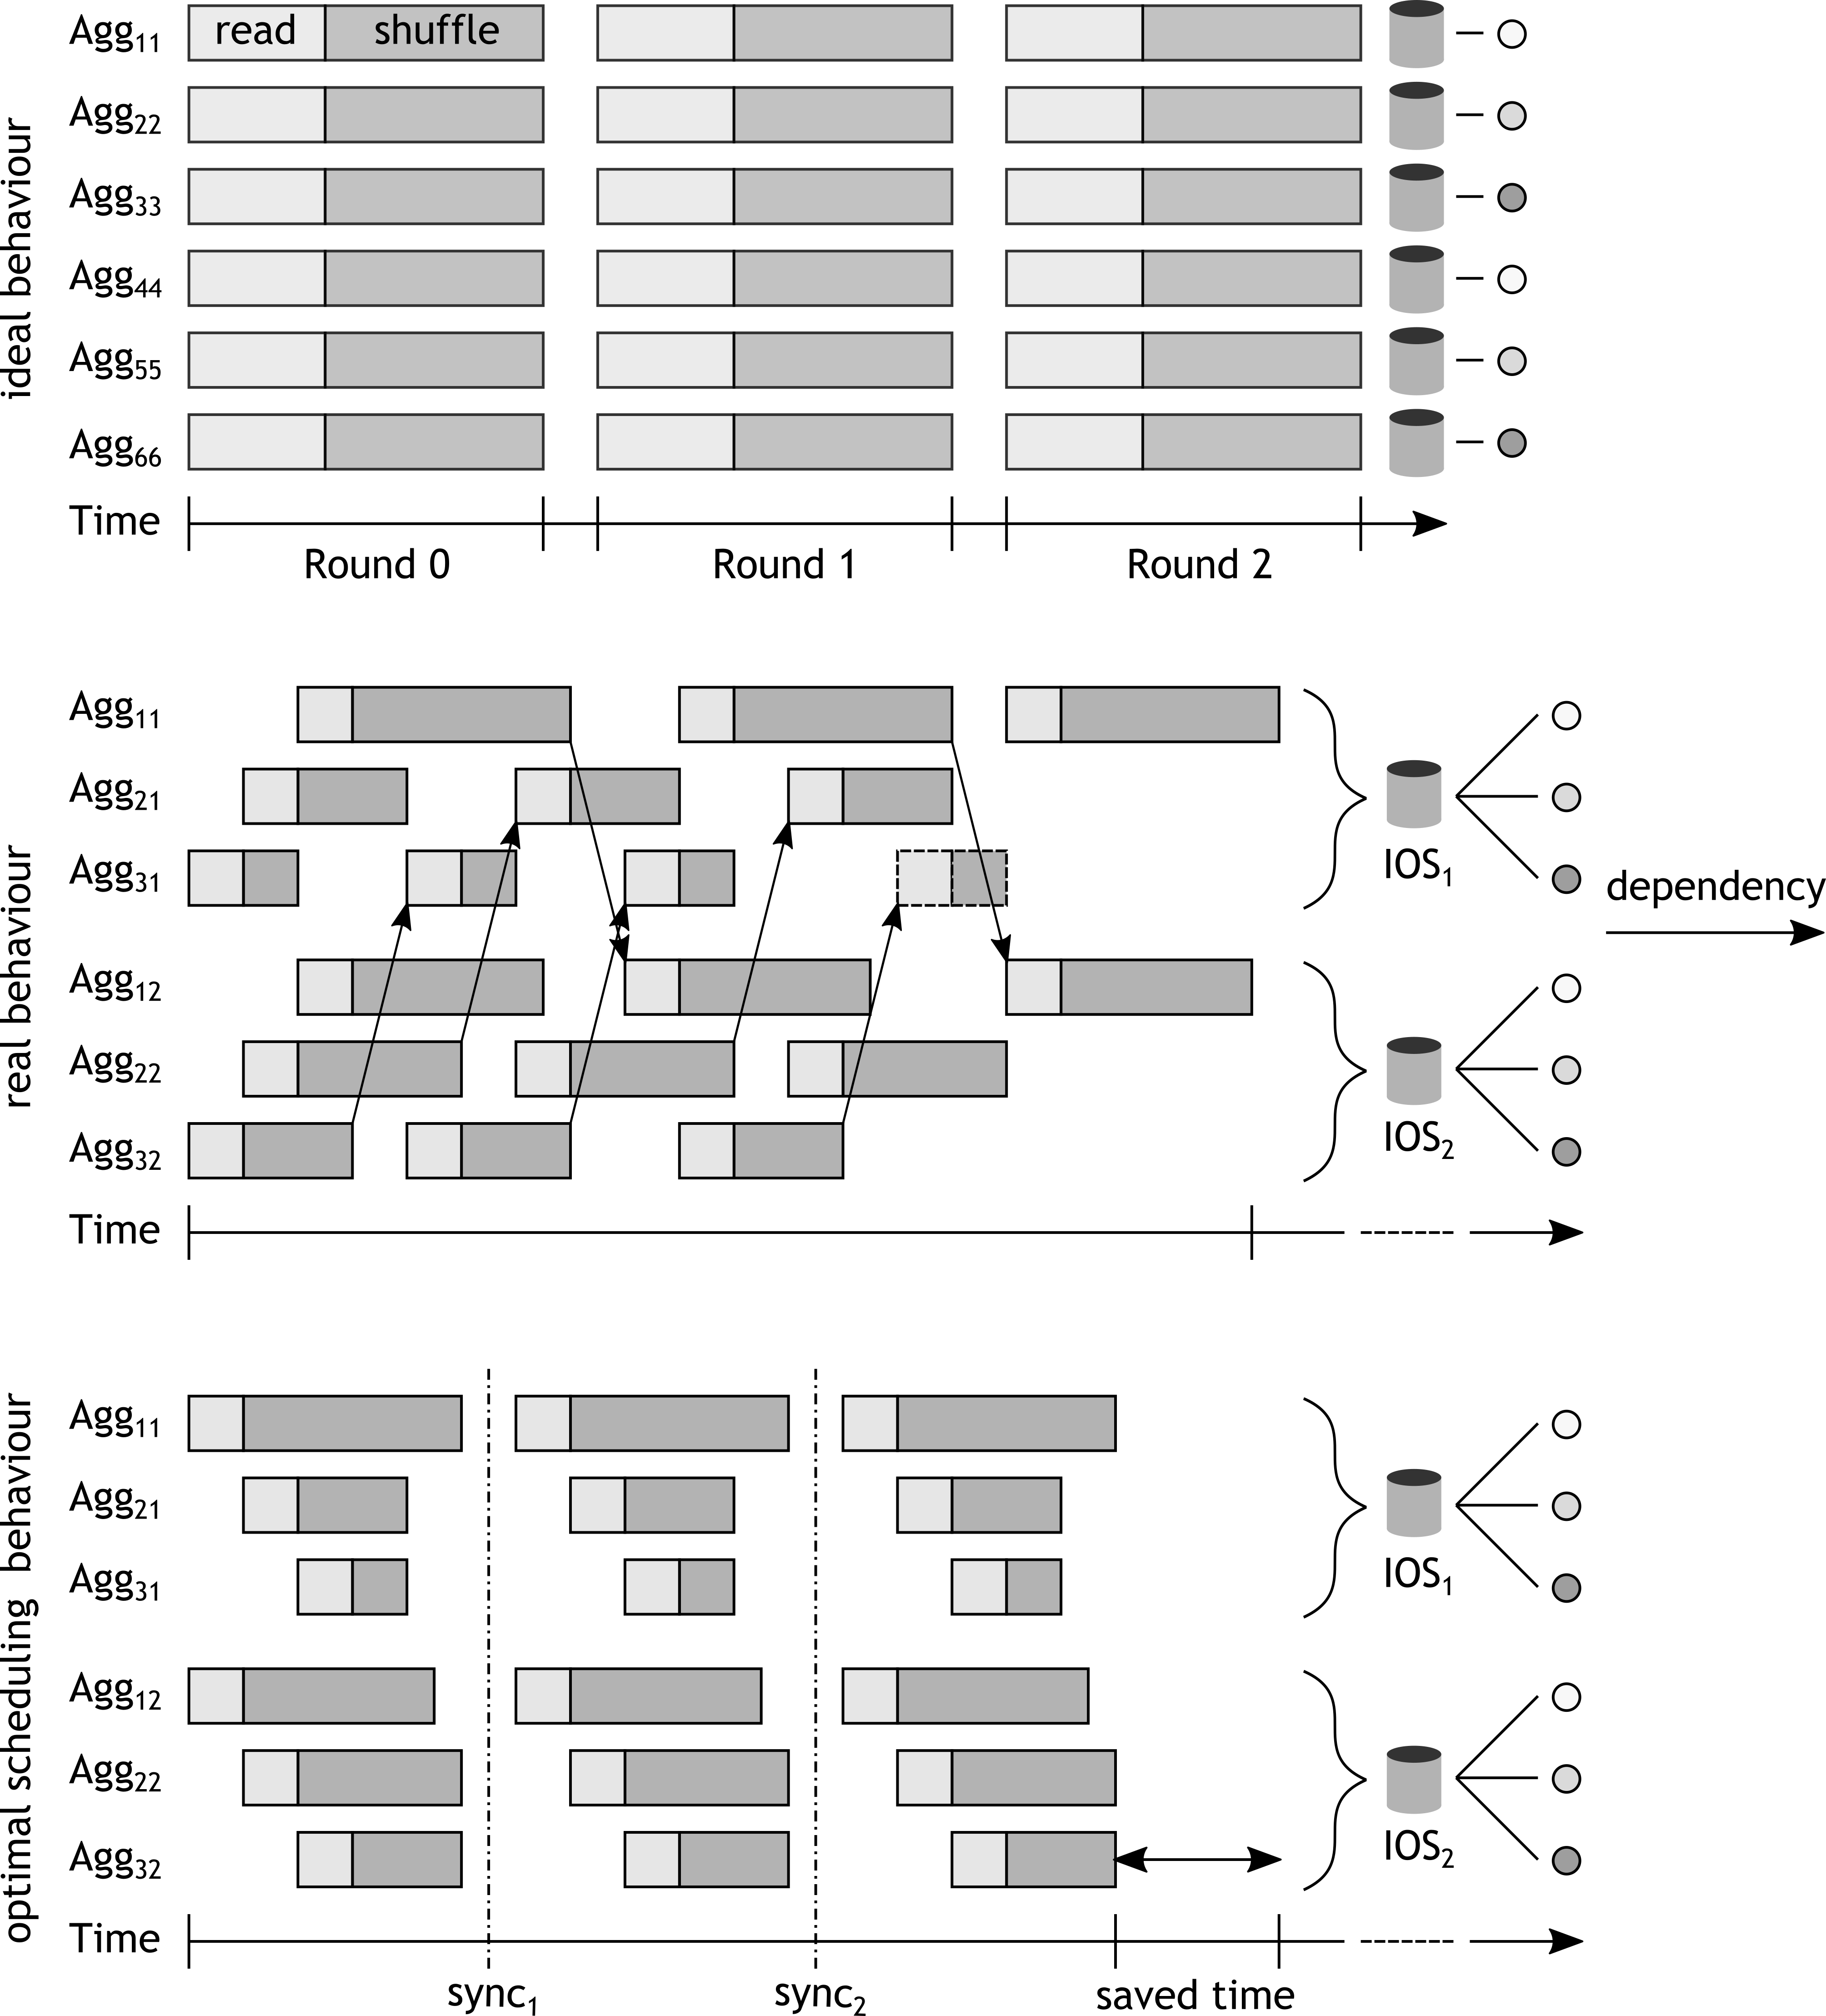
\includegraphics[width=0.8\textwidth]{figures/network-concur}
  \caption{Effect of I/O server scheduling strategies on collective I/O performance. Three examples are shown, in the first every aggregator reads from a different I/O server; in the second three aggregators
  read from the same I/O server, which does not perform any scheduling optimization; and in the third three aggregators read from the same I/O server, which this time does perform a scheduling optimization.}
 % In the figure there are three applications with two aggregators each. In the first example there are six I/O servers. 
 % In the second and third examples there are only two I/O servers, $IOS_1$ and $IOS_2$. $Agg_{11}$ identifies the first aggregator of the first application which reads data from $IOS_1$, $Agg_{12}$ 
 % identifies the second aggregator of the first application which reads data from $IOS_2$, and so on. Every application performs three rounds of two phase I/O. In the `ideal behaviour' every aggregator 
 % reads data from a different I/O server and takes the same time to shuffle data to other processes across the network. In the `real behaviour' aggregators read data only from two I/O servers and take
 % different time to shuffle data. I/O requests in this case are served by arrival order. In the `optimal scheduling behaviour', the slowest aggregator is always served first.}
  \label{figure: network-concur}
\end{figure}

Consider Figure~\ref{figure: network-concur}, showing three applications with two aggregators each and three cases. $Agg_{11}$ identifies the first aggregator of the first application reading data from
$IOS_1$, $Agg_{12}$ identifies the second aggregator of the first application reading data from $IOS_2$, and so on. Every application performs three rounds of two phase I/O. In the `ideal behaviour' every
aggregator reads data from a different I/O server and takes the same time to shuffle data to other processes across the network; in this case all the requests can be ideally scheduled at the same time, giving
the shortest running time for every application. In the `real behaviour' aggregators read data only from two I/O servers and take different time to shuffle data; in this case the shuffle time varies for every
aggregator and is higher for those aggregators that need to exchange data with processes that are placed in a different node\footnote{When aggregators are served by arrival order and the slowest aggregators always
arrive last, the overall collective I/O time dilates.}. In the `optimal scheduling behaviour' the slowest aggregator is always served first; in this case while aggregators are busy shuffling data to other
processes, I/O servers can satisfy following read requests, thus overlapping network communication and I/O time, minimizing the runtime for all applications.
%The first case describes the scenario in which every aggregator requests data from a different 
%I/O server and the shuffle time is the same for each of them. In this case all the requests can be ideally scheduled at the same time giving the shortest running time for every application. The second 
%case describes an example of what the real behaviour may look like. In particular, the shuffle time in this case varies for every aggregator and is higher for aggregators that need to exchange data with 
%processes that are placed in other nodes compared to aggregators that only need to exchange data with processes located in the same node. When aggregators are served by arrival order and slowest aggregators 
%always arrive last, the overall collective I/O time dilates. The third case describes what happens when slowest aggregators are always scheduled first. In this case, while aggregators are busy shuffling 
%data to other processes, I/O servers can satisfy following read requests, thus overlapping network communication time and I/O, minimizing the runtime of all applications.

Liu et al.~\cite{Liu2013} have proposed a new scheduling algorithm for PVFS servers that takes into account the shuffle cost of aggregators across multiple applications and always schedules the slowest
aggregators first, thus achieving the slowest average running time for all of them. This optimization only works for collective read operations. Indeed, for writes the shuffle phase happens before the 
I/O phase. In order to implement the same strategy for write operations, one could use a double buffering approach to pipeline data shuffling and writes. This solution has been proposed by Sehrish et al.
~\cite{Sehrish2013}.

\subsection{Global Synchronization Overhead}
As we have previously discussed in the ext2ph algorithm collective I/O performance is negatively impacted by global synchronization. Collective MPI constructs are used to coordinate processes
in the application and to exchange state during multiple rounds of data shuffling and I/O. Nevertheless, there are cases in which the input domain decomposition, and thus the distribution
of requests in the file, does not require to globally synchronize all processes but only smaller groups of them. These I/O patterns can be exploited to reduce the global synchronization overhead.
Figure~\ref{figure: parcol} shows an example of six processes participating in a collective write operation. In the example there are four aggregators and, as we can see, two groups of three processes
exchange data with only two aggregators.

\begin{figure}[!htb]
  \centering
  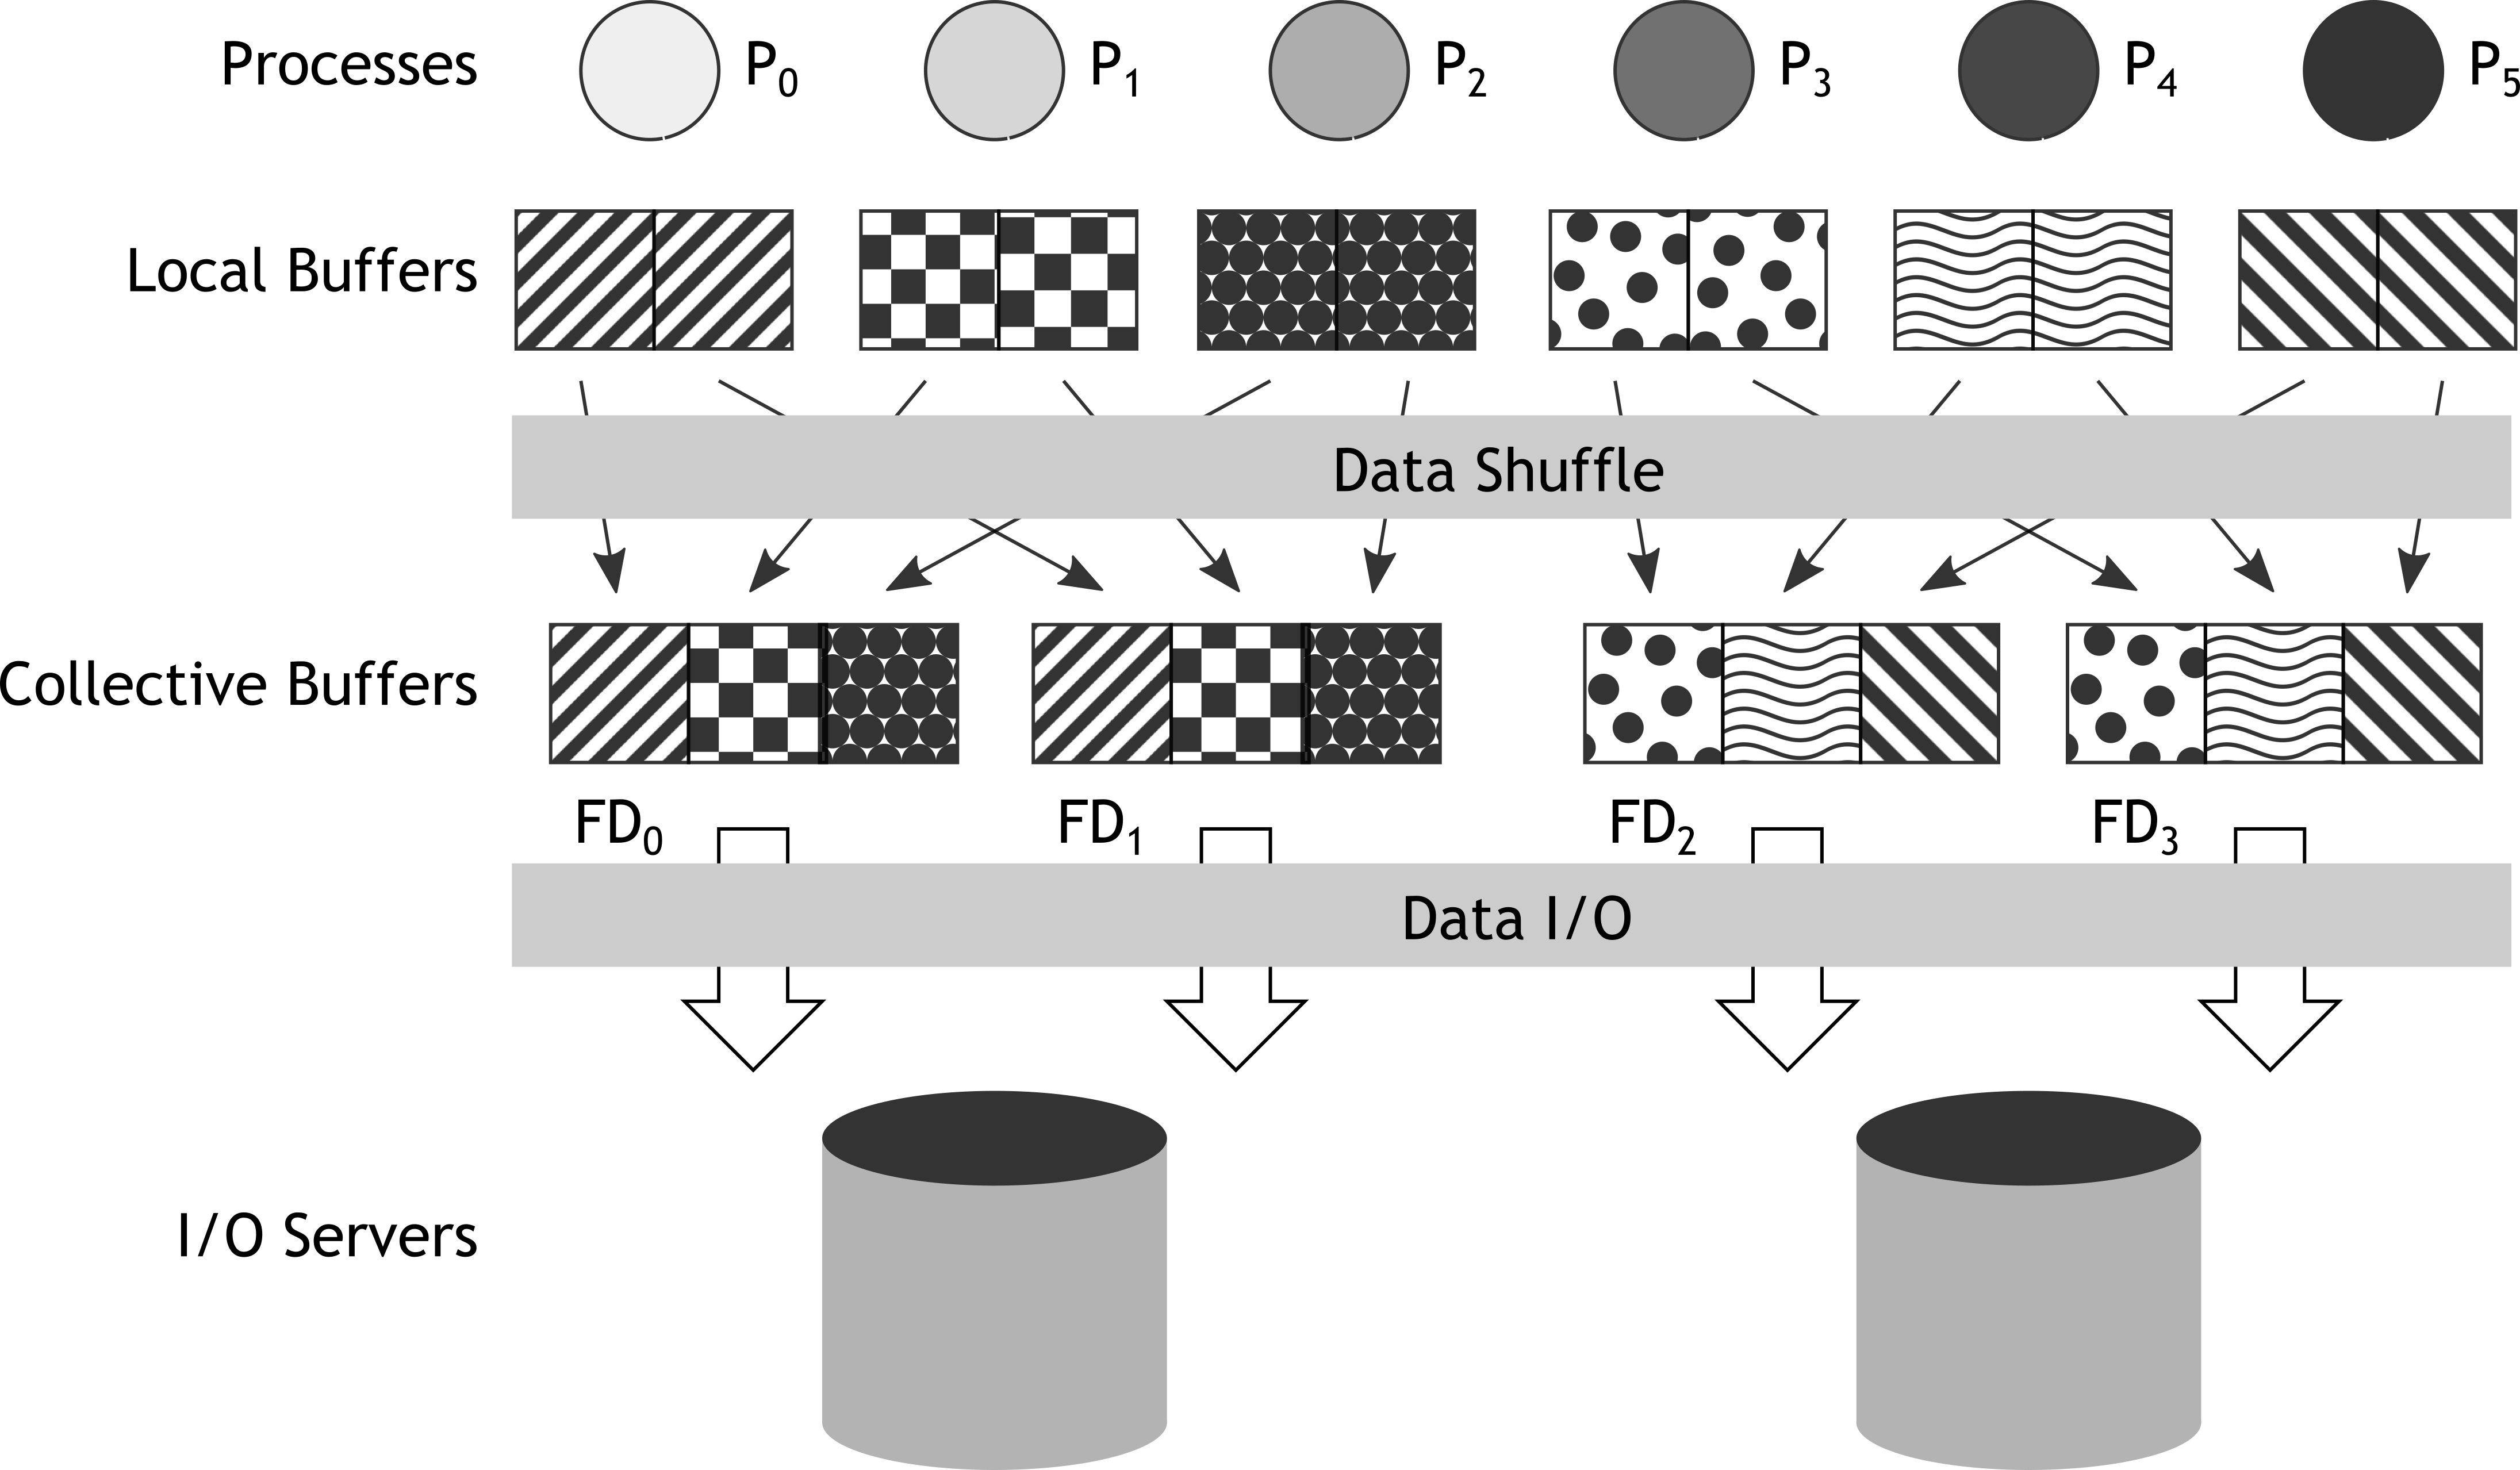
\includegraphics[width=0.8\textwidth]{figures/parcoll}
  \caption{Six processes are collaborating in collective I/O. Because $P_0$, $P_1$ and $P_2$ do not exchange data with other processes there is no need for them to communicate data shuffling information
  to $P_3$, $P_4$ and $P_5$ during two phase I/O rounds.}
  \label{figure: parcol}
\end{figure}

This observation has been exploited by Yu and Vetter~\cite{Yu08} to partition collective I/O into smaller groups of processes that coordinate independently from each other, that is, in the ext2ph
implementation these processes can use different communicators when exchanging data shuffling information with \texttt{MPI\_Alltoall()} (refer to Figure~\ref{figure: coll_io_impl}). Because 
some I/O patterns do not allow the partitioning of processes, they convert the original I/O pattern using an intermediate file view and rearrange data in the file to match the intermediate pattern. This 
approach works but has considerable limitations. In particular, if the file is written using a certain number of processes and aggregators, the original input can be reconstructed only if data in the file 
is read using the same number of processes and aggregators. The reason is that MPI-IO does not define a binary format. Data is written using byte information and in order to reconstruct the intermediate
file view the collective I/O configuration must be the same. The immediate limitation of this approach is that if data is written for checkpoint/restart purposes, the application cannot be restarted using a 
different number of processes because read and write layout would not match.

\section{A Non-Volatile Memory Based Approach} \label{sec: nvm-approach}
As we have discussed in Section~\ref{sec: coll_io_limit}, collective I/O performance is limited by the slowest aggregators run-time. This is mainly due to the fact that the parallel 
file system is shared among many applications in the cluster and requests coming from the same application are not served simultaneously by all I/O servers. This, in conjunction with 
the need for global synchronization at the beginning of every phase of data shuffle and I/O, contributes to the suboptimal performance in large scale clusters. In this work we focus 
on write performance improvements since HPC simulation codes are write intensive; while read operations are typically limited to loading of initialization parameters that are used 
during the simulation. Our approach focuses on global synchronization overhead reduction in the extended two phase algorithm. We achieve our goal by taking advantage of non-volatile 
memory devices, more specifically SSDs, in compute nodes. 

Instead of performing collective I/O to the global parallel file system directly, we perform collective I/O to the local NVM storage and then move data to the global file system asynchronously 
(i.e., in the background), allowing the application to continue with useful work. Data synchronization is not performed collectively but instead independently. This effectively converts collective 
I/O to the parallel file system into independent I/O, taking the parallel file system out of the collective I/O critical path. Since local NVM storage devices are not shared with other nodes, I/O 
requests can be served almost simultaneously, thus reducing the I/O response time in aggregators and limiting the amount of time spent in global synchronization operations. Our approach also benefits 
the memory pressure on compute nodes because we can achieve high performance using smaller collective buffers.

In this section we present the high-level architecture of the ROMIO implementation of MPI-IO as well as our proposed design. The two are shown in Figure~\ref{figure: romio-architecture} 
and~\ref{figure: new-romio-architecture} respectively. The ROMIO middleware is designed to be modular and easily extensible. Support for different parallel file systems is provided through 
additional software modules called drivers. The appropriate driver is selected at file open time through the ADIO interface, following an approach similar to the Virtual File System layer 
of the Linux Kernel.

\begin{figure}[!htb]
  \centering
  \begin{subfigure}[t]{0.38\textwidth}
  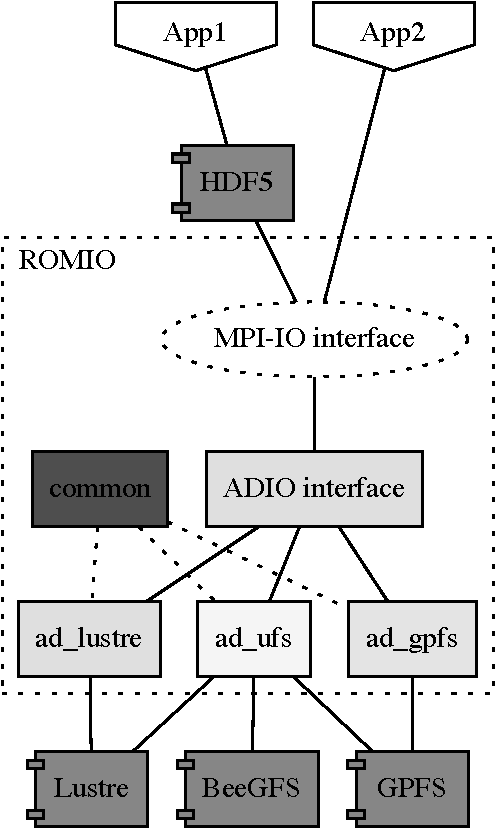
\includegraphics[width=\textwidth]{figures/romio-architecture-baw.pdf}
  \caption{}
  \label{figure: romio-architecture}
  \end{subfigure}
  \begin{subfigure}[t]{0.55\textwidth}
  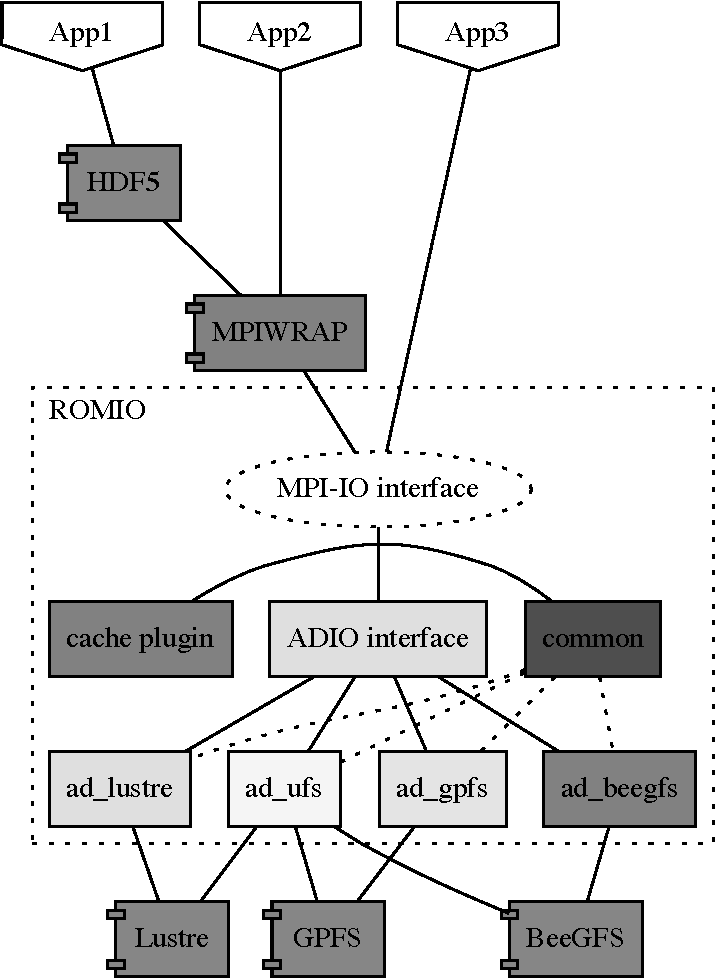
\includegraphics[width=\textwidth]{figures/new-romio-architecture-baw.pdf}
  \caption{}
  \label{figure: new-romio-architecture}
  \end{subfigure}
  \caption{Original ROMIO architecture (\ref{figure: romio-architecture}) and proposed ROMIO architecture (\ref{figure: new-romio-architecture}).}
\end{figure}

In Figure~\ref{figure: romio-architecture} there are three different file system drivers: \textit{ad\_gpfs} for GPFS support, \textit{ad\_ufs} for \textit{universal file system} (UFS) 
support, and \textit{ad\_lustre} for Lustre support. These drivers share features implemented in the \textit{common} module. The common module contains the implementation for most of 
the I/O operations used by the UFS driver (ad\_ufs) and other drivers. File system drivers can implement their own version of I/O operations or use the ones made available by the common 
module. Lustre, for example, uses the common collective open operation (\codeword{ADIOI\_GEN\_Opencoll()}) but implements its own collective write operation (\codeword{ADIOI\_LUSTRE\_WriteStridedColl()}). 
Specific implementations are selected using a file operation table that has to be defined by every file system driver. Listing~\ref{list: lustre_table} shows the operation table for the \textit{ad\_lustre} 
driver.

\begin{lstlisting}[language=C, caption=Operation table for Lustre driver., label={list: lustre_table}]
struct ADIOI_Fns_struct ADIO_LUSTRE_operations = {
    ADIOI_LUSTRE_Open,             /* Open */
    ADIOI_GEN_OpenColl,            /* OpenColl */
    ADIOI_LUSTRE_ReadContig,       /* ReadContig */
    ADIOI_LUSTRE_WriteContig,      /* WriteContig */
    ADIOI_GEN_ReadStridedColl,     /* ReadStridedColl */
    ADIOI_LUSTRE_WriteStridedColl, /* WriteStridedColl */
    ADIOI_GEN_SeekIndividual,      /* SeekIndividual */
    ADIOI_GEN_Fcntl,               /* Fcntl */
    ADIOI_LUSTRE_SetInfo,          /* SetInfo */
    ADIOI_GEN_ReadStrided,         /* ReadStrided */
    ADIOI_LUSTRE_WriteStrided,     /* WriteStrided */
    ADIOI_GEN_Close,               /* Close */
#if defined(ROMIO_HAVE_WORKING_AIO) && !defined(CRAY_XT_LUSTRE)
    ADIOI_GEN_IreadContig,         /* IreadContig */
    ADIOI_GEN_IwriteContig,        /* IwriteContig */
#else
    ADIOI_FAKE_IreadContig,        /* IreadContig */
    ADIOI_FAKE_IwriteContig,       /* IwriteContig */
#endif
    ADIOI_GEN_IODone,              /* ReadDone */
    ADIOI_GEN_IODone,              /* WriteDone */
    ADIOI_GEN_IOComplete,          /* ReadComplete */
    ADIOI_GEN_IOComplete,          /* WriteComplete */
    ADIOI_GEN_IreadStrided,        /* IreadStrided */
    ADIOI_GEN_IwriteStrided,       /* IwriteStrided */
    ADIOI_GEN_Flush,               /* Flush */
    ADIOI_GEN_Resize,              /* Resize */
    ADIOI_GEN_Delete,              /* Delete */
    ADIOI_GEN_Feature,             /* Features */
    "LUSTRE:",
};
\end{lstlisting}

In Figure~\ref{figure: new-romio-architecture} we extend the presented ROMIO architecture with two additional modules: a dedicated driver supporting the BeeGFS file system 
(\textit{ad\_beegfs}) and a \textit{cache plugin} that links directly to the common module, thus providing NVM caching features to all the underlying file system drivers. Indeed,
most of the file system drivers supported in ROMIO use the common implementation of the basic I/O functionalities like, for example, \codeword{ADIOI\_GEN\_OpenColl()} to collectively 
open a file, \codeword{ADIO\_Close()} to collectively close a file, and \codeword{ADIOI\_GEN\_WriteContig()} to write a contiguous extent of data to the file using the POSIX write 
operation. Furthermore, we have also developed an external library called \textit{MPIWRAP} that is used to allow transparent integration of the new caching functionalities into existing 
applications without any need of modifying them. 

\subsection{MPI-IO Hints Extensions}
In order to take advantage of attached non-volatile memories in compute nodes we have introduced a new set of MPI-IO hints, reported in Table~\ref{table: hints_table}, and a 
corresponding set of modifications in the ROMIO implementation of the common layer supporting them.

\begin{table}[!htb]
\centering
\ra{1.5}
\caption{Proposed MPI-IO hints extensions.}
\newcolumntype{K}{>{\centering\arraybackslash} m{4.2cm}}
\newcolumntype{V}{>{\centering\arraybackslash} m{5cm}}
\begin{tabular}{KV}
\toprule
\bf \small Hint & \bf \small Value \\
\midrule
\small \codeword{e10\_cache} & \small \codeword{enable}, \codeword{disable}, \codeword{coherent}\\
\small \codeword{e10\_cache\_path} & \small cache directory pathname\\
\small \codeword{e10\_cache\_flush\_flag} & \small \codeword{flush\_immediate}, \codeword{flush\_onclose}, \codeword{flush\_none}\\
\small \codeword{e10\_cache\_discard\_flag} & \small \codeword{enable}, \codeword{disable}\\
\small \codeword{e10\_cache\_threads} & \small number of synchronization thread in pool\\
\small \codeword{ind\_wr\_buffer\_size} & \small synchronization buffer size [bytes]\\
\hline
\end{tabular}
\label{table: hints_table}
\end{table}

The new hints are used to control the data path in the storage system as well as to define a basic set of cache policies for synchronization and space management. In particular, 
the \codeword{e10\_cache} hint is used to \codeword{enable} or \codeword{disable} the cache, directing applications' data to the local file system instead of the global file system. 
When the hint is set to \codeword{coherent} all the written data extents are locked until cache synchronization is completed. This prevents other processes from modifying the same
data before this is persisted in the global file system. The \codeword{e10\_cache\_path} hint is used to control where, in the local file system tree, the cache file will reside. 
The \codeword{e10\_cache\_flush\_flag} hint is used to control the synchronization policy of cached data to the global file. If the hint is set to \codeword{flush\_immediate} data 
is immediately flushed to the global file. Alternatively, if the hint is set to \codeword{flush\_onclose} data is flushed to the global file when it is closed. A \codeword{flush\_none} 
option is also available to keep data local to the node and never flush it to the global file system. This might be used in the case the user does not wish to flush every checkpoint to the
global file system. The \codeword{e10\_cache\_discard\_flag} hint is used to perform basic cache space management. In particular, if the hint is set to \codeword{enable} the cache file 
is removed after closed, otherwise (\codeword{disable}) it is retained until the user manually removes it. The \codeword{e10\_cache\_threads} hint is used to communicate to the implementation 
the number of threads to be created in the synchronization thread pool when the file is opened (default is 1). Finally, the \codeword{ind\_wr\_buffer\_size} hint controls the size of the 
buffer used to synchronize cached data to the global file. This hint already existed in ROMIO but was only used during independent I/O to determine the write granularity. The hints in 
Table~\ref{table: hints_table} can be used in conjunction with the collective I/O hints described in Table~\ref{table: coll_io_hints_table} of Chapter~\ref{chapt: background}.

Besides the proposed cache policies, more complex ones are possible. For example, the cache synchronization could take into account the level of congestion of the I/O servers. The cache 
replacement policy could also use a more complex strategy to evict cached files (or extents of data inside the file). Although these can be implemented in ROMIO, they introduce more 
sophisticated functionalities that are beyond the scope of this work. Here, our goal is to demonstrate the benefit that the employment of NVM devices in compute nodes can have on parallel
I/O performance.

\subsection{Cache Hints Integration in ROMIO}
As already mentioned, the introduced MPI-IO hints are supported by a corresponding set of modifications in the ROMIO implementation\footnote{\url{http://www.github.com/gcongiu/E10.git}},
which come in the form of cache plugin. The proposed cache plugin class diagram is shown in Figure~\ref{figure: cache-plugin-class}. The cache plugin provides all the functionalities 
necessary to handle the additional cache layer. In the figure there are three main software components: 

\begin{itemize}
\item a synchronization thread object that takes care of moving data from the local to the global file system;
\item a synchronization request object used to describe what data should be moved and finally;
\item an atomic queue object that makes up the communication channel between main and synchronization threads. 
\end{itemize}

In order to handle the cache file properly we have also extended the \codeword{MPI\_File} opaque object with two additional attributes, a cache file handle named \codeword{cache\_fd} and 
an array of pointers to available synchronization thread instances named \codeword{thread\_pool}.

\begin{figure}[!htb]
  \centering
  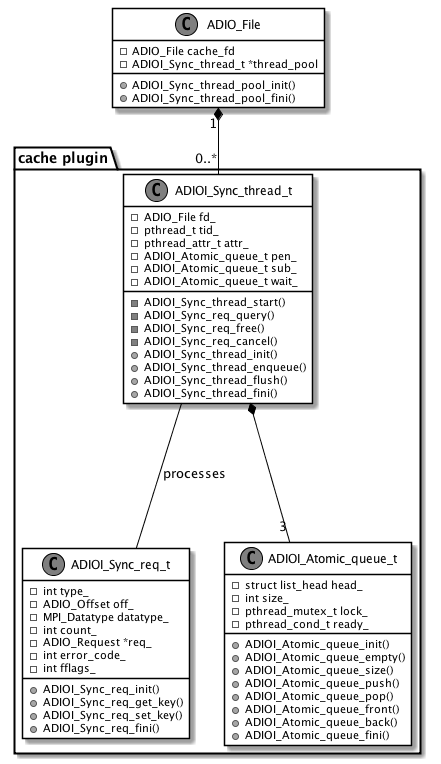
\includegraphics[width=0.6\textwidth]{figures/cache_architecture}
  \caption{Cache plugin class diagram. The synchronization thread \codeword{ADIOI\_Sync\_thread\_t} serves synchronization requests of type \codeword{ADIOI\_Sync\_req\_t}.}
  \label{figure: cache-plugin-class}
\end{figure}

Moreover, we have added two functions, \codeword{ADIOI\_Sync\_thread\_pool\_init()} and \codeword{ADIOI\_Sync\_thread\_pool\_fini()}, to initialize and finalize the thread pool.
In the following we describe in detail the three software components just introduced and explain how they work together.

\subsubsection{Cache Synchronization Thread}
The \codeword{ADIOI\_Sync\_thread\_t} object provides the infrastructure to initialize/finalize threads and to enqueue, flush and wait for synchronization requests. A pool of synchronization threads 
is created when the file is opened with \codeword{MPI\_File\_open()} and destroyed when the file is closed with \codeword{MPI\_File\_close()}. The synchronization thread object has six attributes: 
the \codeword{fd\_} attribute is a pointer to the internal ROMIO representation of the MPI file object and is used by the thread to retrieve all the information it requires to perform its tasks 
(e.g., POSIX file descriptors) without having to pass such information through the synchronization request object; the \codeword{tid\_} attribute is the POSIX thread identifier and is used by the 
main thread in the \codeword{pthread\_join()} operation when the file is closed; the \codeword{attr\_} are the POSIX thread attributes; finally there are three queues, a submission queue named 
\codeword{sub\_} that contains requests that are ready to be served, a pending queue named \codeword{pen\_} that contains requests that are not yet ready to be served, and a wait queue named 
\codeword{wait\_} that contains a copy of every request that is in the submission queue and is used by the main thread to check status of submitted requests.

%\begin{lstlisting}[language=C, caption=Synchronization Thread API, label={list: sync-thread}]
%%/* Used by ADIOI_Sync_req_init() method */
%enum {
%  ADIOI_THREAD_SYNC = 0,
%  ADIOI_THREAD_SHUTDOWN
%};
%
%/* Synchronization Thread Object Definition */
%struct ADIOI_Sync_thread {
%  ADIO_File            fd_;
%  pthread_t            tid_;
%  pthread_attr_t       attr_;
%  ADIOI_Atomic_queue_t sub_;
%  ADIOI_Atomic_queue_t pen_;
%  ADIOI_Atomic_queue_t wait_;
%};
%
%/* Synchronization Thread Opaque Object */
%typedef struct ADIOI_Sync_thread *ADIOI_Sync_thread_t;
%
%/* Synchronization Thread Public APIs */
%int  ADIOI_Sync_thread_init(ADIOI_Sync_thread_t *, ...);
%int  ADIOI_Sync_thread_fini(ADIOI_Sync_thread_t *);
%void ADIOI_Sync_thread_enqueue(ADIOI_Sync_thread_t, ADIOI_Sync_req_t);
%void ADIOI_Sync_thread_flush(ADIOI_Sync_thread_t);
%void ADIOI_Sync_thread_wait(ADIOI_Sync_thread_t);
%\end{lstlisting}

The public interface of the synchronization thread provides two methods to initialize and destroy the thread object and three additional methods: \codeword{ADIOI\_Sync\_thread\_enqueue()} used by 
the main thread to enqueue new requests in the pending queue, \codeword{ADIOI\_Sync\_thread\_flush()} used by the main thread to move requests from the pending queue to the submission queue, thus
allowing the thread to serve them, and finally \codeword{ADIOI\_Sync\_thread\_wait()} used by the main thread to wait for all the submitted requests to complete. The thread object also contains
four additional internal methods that are not directly visible to the main thread and are used to implement the supported services through the MPI generalized request interface~\cite{mpispecs}.

\subsubsection{Cache Synchronization Request}
The \codeword{ADIOI\_Sync\_req\_t} object provides the infrastructure required to initialize/finalize, set/get attributes to/from synchronization requests. Synchronization requests are initialized 
by the main thread in the \codeword{ADIO\_GEN\_WriteContig()} function and submitted to synchronization threads which will satisfy them while the main thread can progress with its work. 
The synchronization request object has seven attributes: the \codeword{type\_} attribute specifies the type of the request, either \codeword{ADIOI\_THREAD\_SYNC} or \codeword{ADIOI\_THREAD\_SHUTDOWN};
the first is used to describe a written file extent that needs to be copied from the cache to the global file system, while the second is used to shut down the synchronization thread when the thread 
is no longer needed; the \codeword{count\_} attribute represents the number of elements of type \codeword{datatype\_} to be transfered, while the initial position of these in the file is defined
by the \codeword{offset\_} attribute; the \codeword{fflags\_} attribute tells the synchronization thread when data should be transfered; the \codeword{req\_} attribute is a MPI request handle and is 
used by the main thread to check the synchronization status of the request by invoking \codeword{MPI\_Wait()}; finally, the \codeword{error\_code\_} attribute is used by the synchronization thread to 
set the return code that is afterwards interpreted by the main thread.

%\begin{lstlisting}[language=C, caption=Synchronization Request Attributes and Public API., label={list: sync-req}]
%/* Used by ADIOI_Sync_req_{get,set}_key() methods */
%enum {
%  ADIOI_SYNC_TYPE = 0, /* sync req type        */
%  ADIOI_SYNC_OFFSET,   /* sync req write off   */
%  ADIOI_SYNC_DATATYPE, /* sync req datatype    */
%  ADIOI_SYNC_COUNT,    /* sync req count       */
%  ADIOI_SYNC_REQ,      /* sync req MPI_Request */
%  ADIOI_SYNC_ERR_CODE, /* sync req error_code  */
%  ADIOI_SYNC_FFLAGS,   /* sync req flush flag  */
%  ADIOI_SYNC_ALL,      /* sync req all fields  */
%  ADIOI_SYNC_REQ_ERR   /* sync req err code    */
%};
%
%/* Synchronization Request Object Definition */
%struct ADIOI_Sync_req {
%  int           type_;
%  int           count_;
%  int           error_code_;
%  int           fflags_;
%  ADIO_Offset   off_;
%  MPI_Datatype  datatype_;
%  MPI_Request  *req_;
%};
%
%/* Synchronization Request Opaque Object */
%typedef struct ADIOI_Sync_req *ADIOI_Sync_req_t;
%
%/* Synchronization Request Public APIs */
%int ADIOI_Sync_req_init(ADIOI_Sync_req_t *, ...);
%int ADIOI_Sync_req_fini(ADIOI_Sync_req_t *);
%int ADIOI_Sync_req_get_key(ADIOI_Sync_req_t, ...);
%int ADIOI_Sync_req_set_key(ADIOI_Sync_req_t, ...);
%\end{lstlisting}

The public interface of the synchronization request object provides two methods to initialize and destroy the synchronization request object, a get method named \codeword{ADIOI\_Sync\_req\_get\_key()} 
and a set method named \codeword{ADIOI\_Sync\_req\_set\_key()}. 

\subsubsection{Atomic Queue}
The \codeword{ADIOI\_Atomic\_queue\_t} object provides the communication channel between the main thread and the synchronization thread enforcing atomicity through POSIX mutual exclusion constructs.
The atomic queue object has four attributes: the \codeword{head\_} attribute is a pointer to the head of a double linked list used to implement the queue\footnote{We used the Linux kernel implementation
of the double linked list.}; the \codeword{size\_} stores the number of elements currently present in the queue; the \codeword{lock\_} attribute is a POSIX mutex used to ensure internal data structure 
consistency during queue manipulation; finally, the \codeword{ready\_} attribute is a condition variable used by the main thread to signal the synchronization thread that the queue is no longer empty. 

%\begin{lstlisting}[language=C, caption=Atomic Queue Attributes and Public API., label={list: atomic-queue}]
%/* Atomic Queue Object Definition */
%struct ADIOI_Atomic_queue {
%  struct list_head head_;
%  int              size_;
%  pthread_mutex_t  lock_;
%  pthread_cond_t   ready_;
%};
%
%/* Atomic Queue Opaque Object */
%typedef struct ADIOI_Atomic_queue *ADIOI_Atomic_queue_t;
%
%/* Atomic Queue Public APIs */
%void ADIOI_Atomic_queue_init(ADIOI_Atomic_queue_t *);
%void ADIOI_Atomic_queue_fini(ADIOI_Atomic_queue_t *);
%int  ADIOI_Atomic_queue_empty(ADIOI_Atomic_queue_t);
%int  ADIOI_Atomic_queue_size(ADIOI_Atomic_queue_t);
%ADIOI_Sync_req_t ADIOI_Atomic_queue_front(ADIOI_Atomic_queue_t);
%ADIOI_Sync_req_t ADIOI_Atomic_queue_back(ADIOI_Atomic_queue_t);
%void ADIOI_Atomic_queue_push(ADIOI_Atomic_queue_t,   ADIOI_Sync_req_t);
%void ADIOI_Atomic_queue_pop(ADIOI_Atomic_queue_t);
%\end{lstlisting}

The atomic queue object supports the standard queue APIs\footnote{http://www.cplusplus.com/reference/queue/queue/?kw=queue} and thus we do not give a description for them here.

\subsubsection{Collective Write Caching}
Now that we have described all the cache plugin components, we can explain how the cache plugin works in collective write operations. Figure~\ref{figure: coll_io_cache} shows the flow diagram
obtained by extending the diagram in Figure~\ref{figure: coll_io_impl} with the cache plugin. 
\begin{figure}[H]
  \centering
  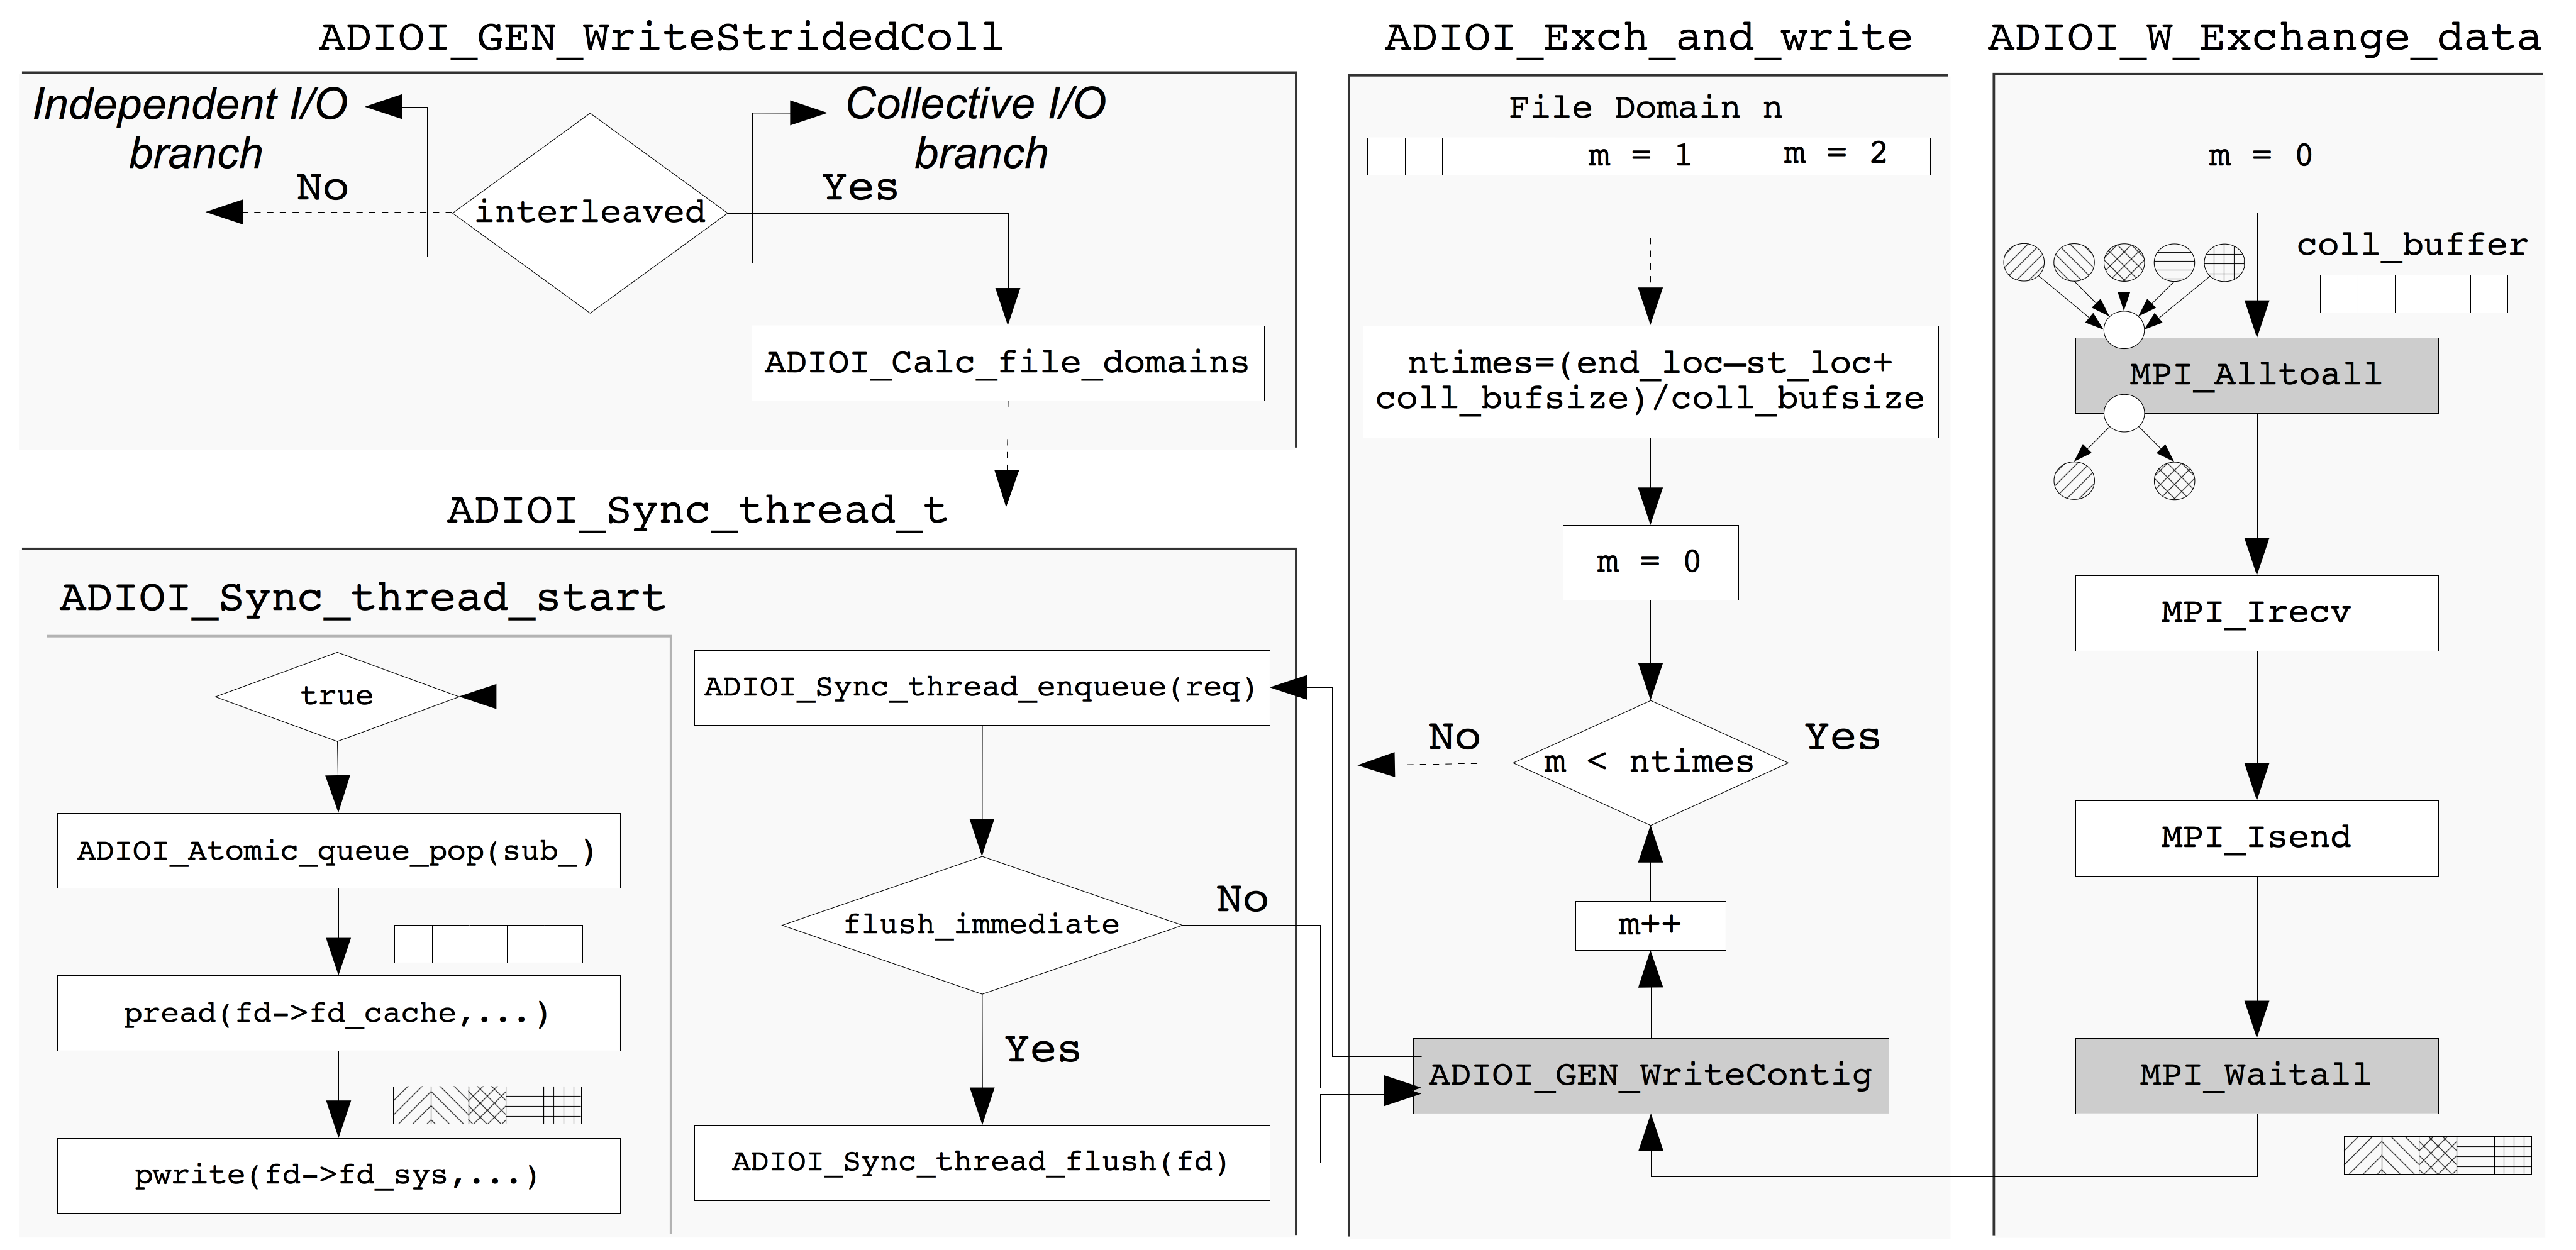
\includegraphics[angle=90,width=0.8\textwidth]{figures/ext2ph+e10_t}
  \caption{Extended collective I/O flow diagram including cache plugin support.}
  \label{figure: coll_io_cache}
\end{figure}
The first part of the diagram in the upper left part is left unchanged. The changes are introduced in the \codeword{ADIO\_GEN\_WriteContig()}\footnote{In the BeeGFS driver this is replaced by 
\codeword{ADIOI\_BEEGFS\_WriteContig()}.} operation. This has been modified to redirect writes to the local file system cache whenever the cache is enabled, that is, when the \codeword{e10\_cache} 
hint is set to enable. After data is written to the cache, the function creates a new synchronization request of type \codeword{ADIOI\_THREAD\_SYNC} by invoking \codeword{ADIOI\_Sync\_req\_init()} 
and enqueues it into the pending queue of the synchronization thread through \codeword{ADIOI\_Sync\_thread\_enqueue()}. At this point the main thread also checks the desired flushing policy defined by 
the \codeword{e10\_cache\_flush\_flag} hint. If the hint is set to \codeword{flush\_immediate} the main thread immediately flushes the enqueued requests to the submission queue by invoking 
\codeword{ADIOI\_Sync\_thread\_flush()} and then returns. Otherwise requests are left in the pending queue and will be served when the file is closed with \codeword{MPI\_File\_close()} or when the 
main thread invokes \codeword{MPI\_File\_sync()}.

\subsection{BeeGFS Cache Integration in ROMIO}
The BeeGFS file system provides its own caching infrastructure, which includes a set of APIs to control the caching functionalities and a daemon process, running on the host machine, that takes care of 
moving data between the cache and the global file system. For this reason, some of the cache plugin features presented before for the universal file system module in the common layer are redundant. In 
particular, we do not any longer need to manually open a cache file in the host and start a pool of synchronization threads. When using the BeeGFS cache API the file system takes care of all these aspects 
for us. Nevertheless, we still reused some parts of the cache plugin to integrate the BeeGFS cache support into ROMIO. For more details about the cache implementation in the BeeGFS driver refer to the
source code at http://www.github.com/gcongiu/E10.git.

\subsection{Consistency Semantics}
As far as write consistency semantic is concerned, the MPI-IO interface does not make any assumption regarding the underlying parallel file system or its semantics. ROMIO specifically supports file systems that are 
both POSIX compliant, like Lustre, and non-POSIX compliant, like NFS or PVFS. In MPI-IO, written data becomes globally visible only after either \codeword{MPI\_File\_sync()} or \codeword{MPI\_File\_close()} 
are invoked on the MPI file handle and by default there is no write atomicity. The motivation is that data can be cached at some level locally in the compute nodes. The ROMIO implementation can overcome the 
risk of data inconsistency, e.g., related to false sharing of file system blocks, using persistent file realms~\cite{ColomaCWWRP04}, and can even enforce atomicity using \codeword{MPI\_File\_set\_atomicity()}.

In our implementation we comply to the MPI-IO semantics just described. This means that data written to the local file system cache using the newly introduced MPI-IO hints will be globally visible to the rest 
of the nodes only under the following circumstances:

\begin{itemize}
\item The \codeword{e10\_cache\_flush\_flag} has been set to \codeword{flush\_immediate} by the user and synchronization, started automatically by the implementation right after the write operation, has completed;
\item The \codeword{e10\_cache\_flush\_flag} has been set to \codeword{flush\_onclose} by the user and the invoked \codeword{MPI\_File\_close()} has returned;
\item The \codeword{MPI\_File\_sync()} function has been invoked by the user and it has returned.
\end{itemize}

Consistency for reading data from the cache is not clearly defined by the ext2ph algorithm. In general, data written to the local file system cache can be read back from the user without accessing the global 
file system. However, the algorithm calculates the location of a data block based on the number of aggregators, their logical position within the set of aggregators, and the size of the complete data set. 
This means that a collective read that matches the previous write could safely retrieve the data from the aggregators' cache without incurring into any problem. In spite of that, in general reading from the 
cache requires additional metadata describing the file layout across the caches. For this reason, we currently do not support reads from the local file system cache.

Furthermore, whenever required, we can enforce cache coherency ensuring that read operations cannot access data that is currently in transit, i.e., not or only partially moved from the cache to the global file. 
This can be done by locking the file domain extent being cached until all the data has been made persistent in the global file. For this purpose ROMIO provides a set of internal locking macros, namely 
\codeword{ADIOI\_WRITE\_LOCK}, \codeword{ADIOI\_READ\_LOCK} and \codeword{ADIOI\_UNLOCK} that we used in our implementation. The lock of cached data can be selected by setting the \codeword{e10\_cache} hint in 
Table~\ref{table: hints_table} to \codeword{coherent}. This will \codeword{enable} the cache and set locks appropriately, assuming underlying file system support.

\subsection{Changes to the Application's Workflow}
Simplifying, most HPC simulation codes can be divided into multiple phases of computation, in which data is produced, and I/O, in which data is written to persistent storage for post-processing purposes as well as 
defensive checkpoint/restart. Focusing on the I/O phase and considering the case of applications writing to a shared file, the I/O phase can be divided into the following steps:

\begin{enumerate}
\item The file is opened using \codeword{MPI\_File\_open()}: at this point the info object containing the user defined MPI-IO hints is passed to the underlying ROMIO layers;
\item Data is written to the file using \codeword{MPI\_File\_write\_all()}: this function invokes the underlying \codeword{ADIOI\_GEN\_WriteStridedColl()} previously described in Figure~\ref{figure: coll_io_impl};
\item The file is closed using \codeword{MPI\_File\_close()}: after the file is closed data must be visible to every process in the cluster. 
\end{enumerate}

To take advantage of the proposed MPI-IO hint extensions, the application's workflow has to be modified. Figure~\ref{figure: workflow} shows the classical application's workflow (cache disabled) as well as the modified 
version using the new hints (cache enabled). The difference is that, in order to take advantage of the proposed hints and hide the cache synchronization to the computation phase, the \codeword{MPI\_File\_close()} for the 
I/O phase \textit{k} has been moved at the beginning of the I/O phase \textit{k+1}, just before the new file is opened.

\begin{figure}[!htb]
  \centering
  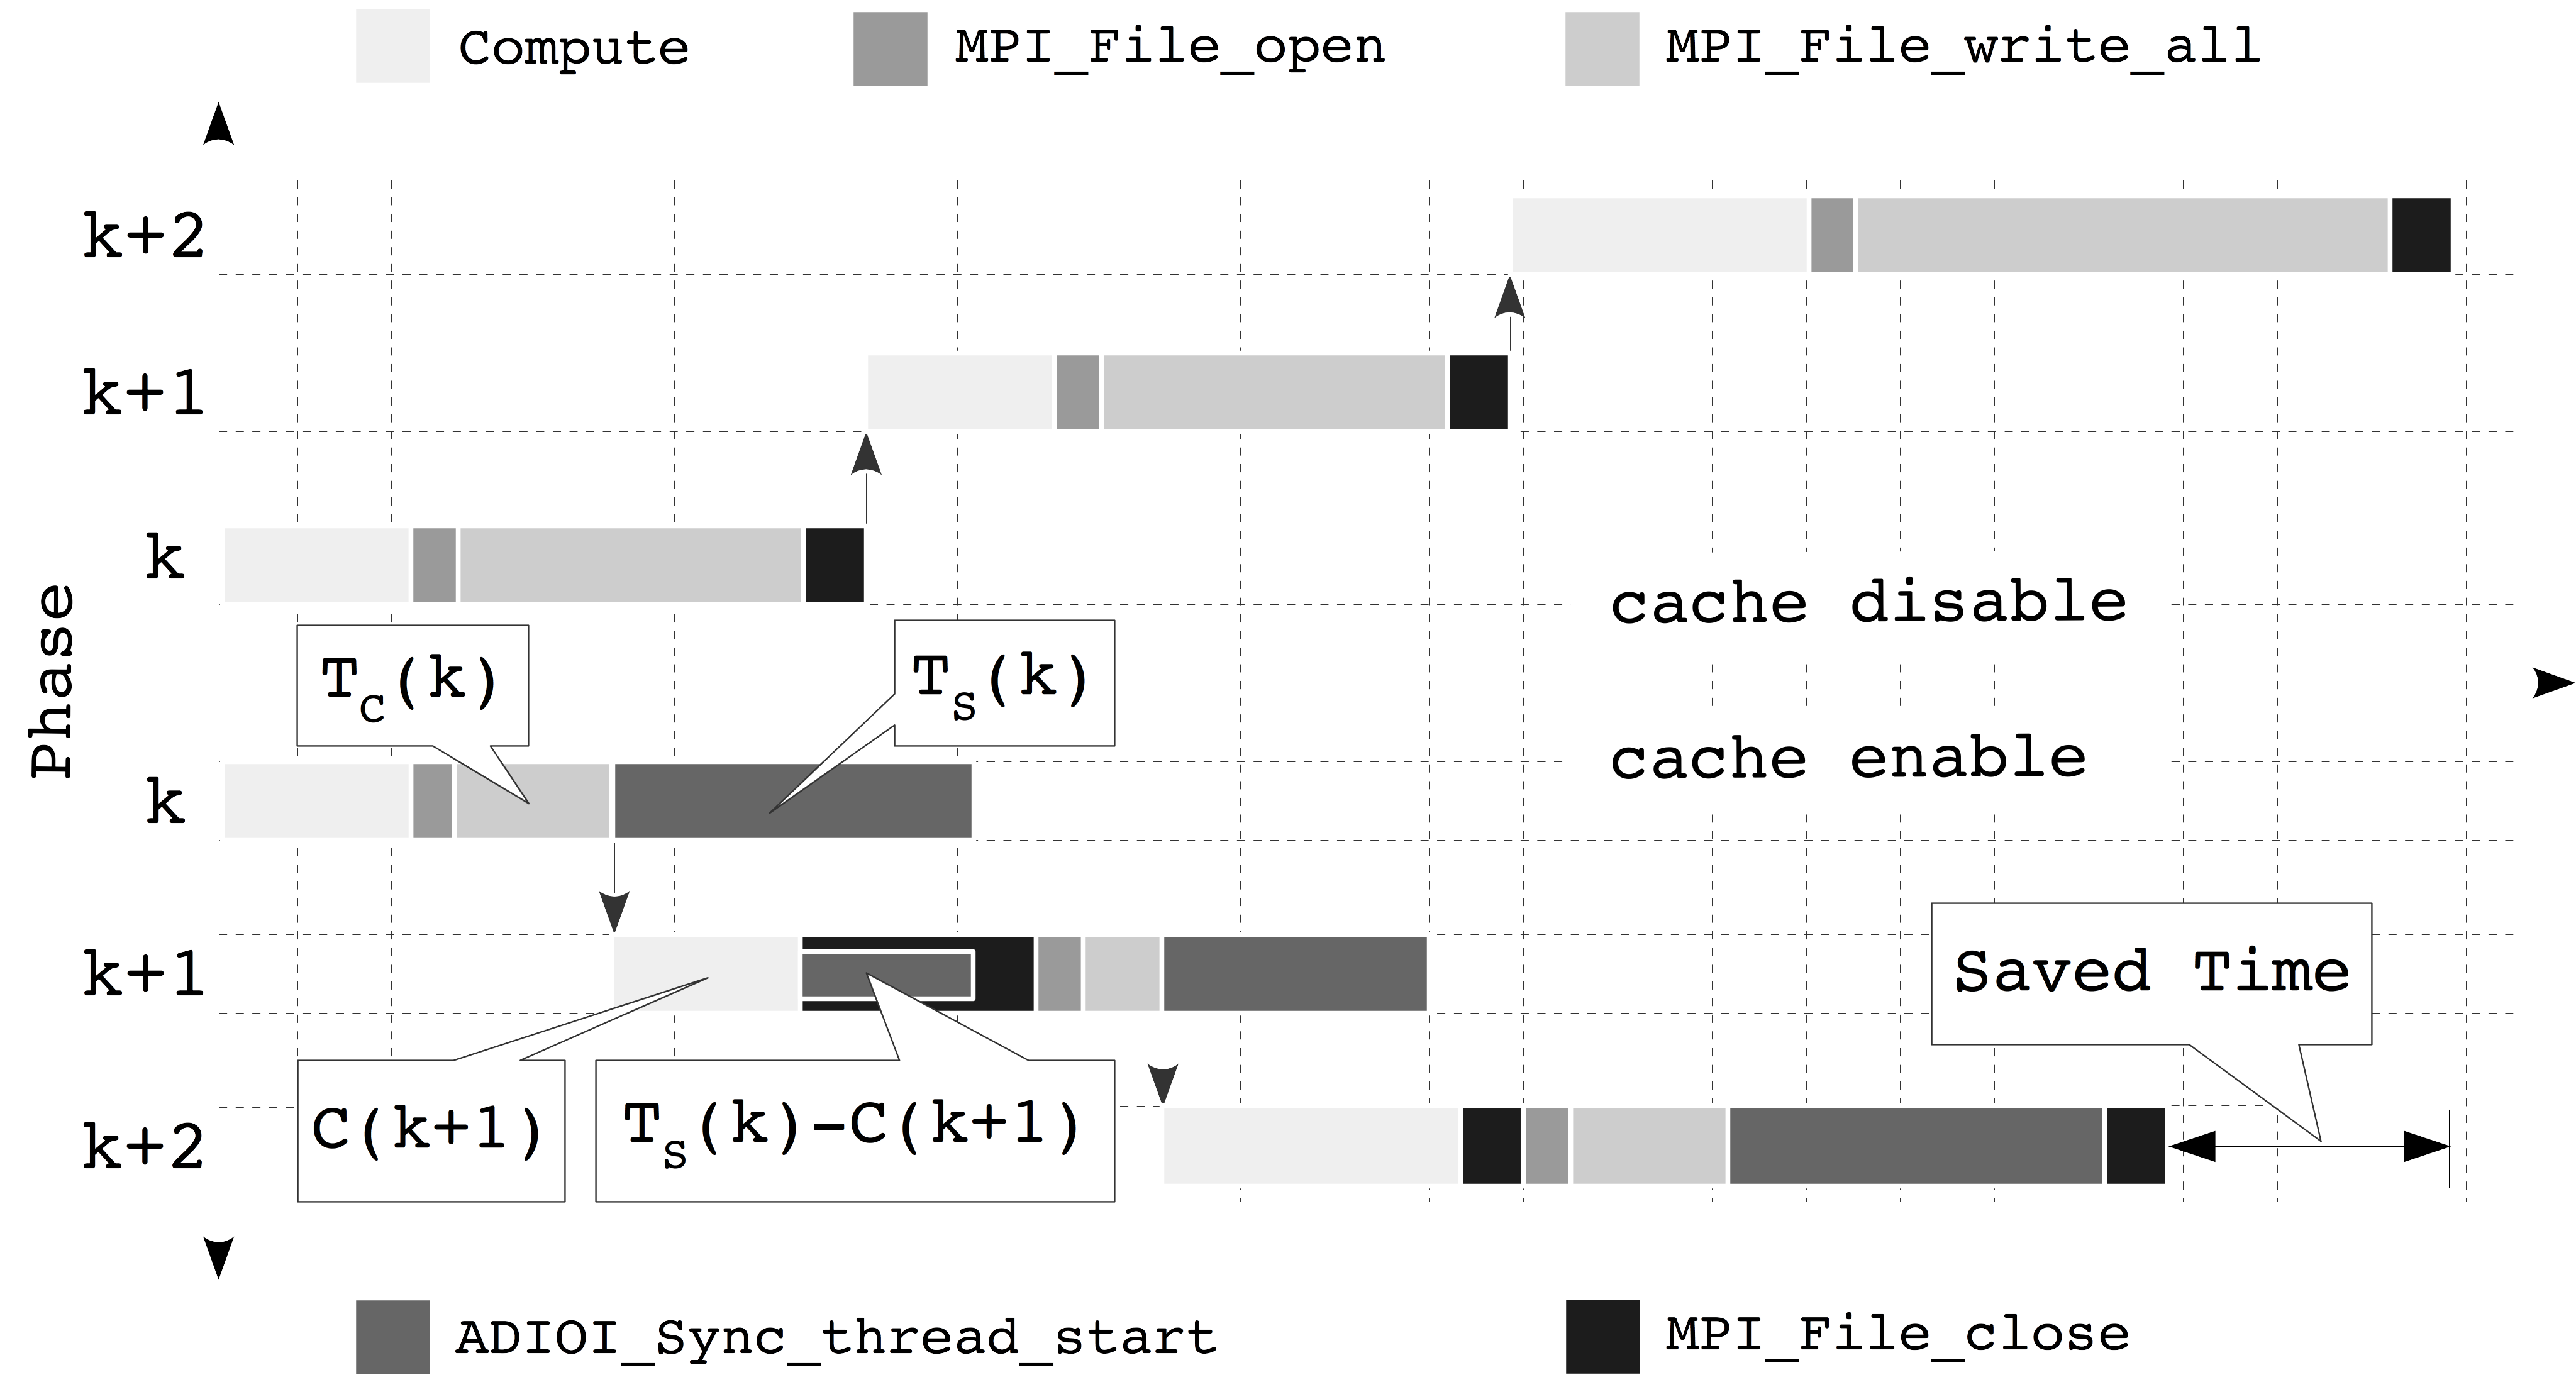
\includegraphics[width=0.9\textwidth]{figures/workflow_baw}
  \caption{Standard and modified workflows. When cache is disabled compute phase `k+1' starts after file `k' has been closed. 
  When the cache is enabled compute `k+1' can start immediately after data has been written. At the same time, background 
  synchronization of cached data starts. File `k' is closed before the file `k+1' is opened, forcing the implementation to wait 
  for cache synchronization to complete.}
  \label{figure: workflow}
\end{figure}

\subsubsection{MPIWRAP Library}
Since the workflow modification just presented might not be feasible for legacy applications, we developed a MPI-IO wrapper library (called MPIWRAP), written in C++, that can reproduce this change behind the scenes. 
The library can be linked to the application or preloaded with \codeword{LD\_PRELOAD} and has been used for all the experiments contained in this thesis. MPI-IO hints are defined in a configuration file and passed 
by the library to \codeword{MPI\_File\_open()}. We can define multiple hints targeting different files or groups of files. The library overloads \codeword{MPI\_\{Init,Finalize\}()} and \codeword{MPI\_File\_\{open,close\}()} 
using the PMPI profiling interface. The workflow modification can be triggered for a specific set of files (identified by the same base name) in the configuration file. Whenever one of such files is closed, our \codeword{MPI\_File\_close()} 
implementation will return success. However, the file will not be really closed. Instead, its handle will be kept internally for future references. When the next shared file with the same base name is opened, our 
\codeword{MPI\_File\_open()} implementation will search for outstanding opened file handles and will invoke \codeword{PMPI\_File\_close()} on them before opening the new file, thus triggering the cache synchronization 
completion check for each of them.

\subsection{Write Bandwidth}
According to the new I/O workflow, described in this section, we have that being $S(k)$ the amount of data written during phase \textit{k}, $T_c(k)$ the time needed to write $S(k)$ collectively to the cache using 
\codeword{MPI\_File\_write\_all()}, $T_s(k)$ the time needed to synchronise the cached data in every aggregator to the global file system (through \codeword{ADIOI\_Sync\_thread\_start()}), and $C(k+1)$ the 
computation time of phase \textit{k+1}, the resulting write bandwidth for \textit{k} is expressed by Equation~\ref{formula: bw}:

\begin{equation}\label{formula: bw}
        bw(k) = \frac{S(k)}{T_c(k) + max(0,\ T_s(k) - C(k+1))}
\end{equation}
Therefore, the total average bandwidth perceived by the application is:
\begin{equation}\label{formula: abw}
        BW = \frac{\sum_{k=0}^{N-1} S(k)}{\sum_{k=0}^{N-1} T_c(k) + max(0,\ T_s(k) - C(k+1))}
\end{equation}

From Equation~\ref{formula: bw} (in which we have considered the open time neglectable) it is clear that the maximum performance can be obtained when $C(k+1) \geq T_s(k)$, that is, when we can completely hide 
cache synchronization to the computation phase. On the other hand when $C(k+1) < T_s(k)$ we might have a minima in the bandwidth since \codeword{MPI\_File\_close()} needs to wait for cache synchronization 
completion (Figure~\ref{figure: workflow}). 

\section{Contributions} \label{sec: nvm-related}
Many research works have tried to optimize collective I/O focusing on different aspects. Yu and Vetter~\cite{Yu08} before us have identified the global synchronization 
problem as one of the most severe for collective I/O performance. They exploited access pattern characteristics, common in certain scientific workloads, to partition collective 
I/O into smaller communication groups and synchronise only within these. Block-tridiagonal patterns, not directly exploitable, are automatically reduced, through an intermediate 
file view, to a more manageable pattern and can thus take advantage of the proposed solution. The ADIOS library~\cite{Lofstead2008} addresses this problem similarly by dividing a 
single big file into multiple files to which collective I/O is carried out independently for separated smaller groups of processes. 

Lu et al.~\cite{Lu2012}~\cite{Lu2013} further explored collective I/O performance beyond global synchronization and considered memory pressure of collective I/O buffers. They proposed 
a memory conscious implementation that accounts for reduced memory per core in future large scale systems. Liao~\cite{Liao11} focused on the file domain partitioning impact on parallel 
file systems' performance. He demonstrated that by choosing the right file domain partitioning strategy, matching the file system locking protocol, collective write performance can be 
greatly improved.

Chen et al.~\cite{Chen2011} addressed the problem of I/O server contention using a layout aware strategy to reorganize data in aggregators. On the same lines, 
Xuechen et al.~\cite{Zhang2009} proposed a strategy to make collective I/O `resonant' by matching memory layout and physical placement of data in I/O servers and exploiting 
non-contiguous access primitives of PVFS. The strategy proposed is similar in concept to the Lustre implementation of collective I/O in which file contiguous patterns are converted to 
stripe contiguous patterns and the concurrency level on OSTs can be set using the MPI-IO hint \codeword{romio\_lustre\_co\_ratio} (Client-OST ratio). 

Liu et al.~\cite{Liu2013} exploited the scheduling capabilities of PVFS I/O servers to rearrange I/O requests' order and better overlap read and shuffle phases among different processes. 
Yu et al.~\cite{Yu2007} used the file joining functionalities of Lustre to convert collective I/O into independent I/O to multiple files, thus avoiding file system stripe contention. All 
resulting files are afterwards rejoined into a single shared file.

Lee et al.~\cite{LeeRTXW04} proposed RTS as infrastructure for remote file access and staging using MPI-IO. Similarly to our approach, RTS uses additional threads, 
Active Buffering Threads (ABT)~\cite{XiaosongWLS03}, to transfer data in background to the compute phase. Moreover, the authors also modified the ABT ROMIO driver implementation to stage data in 
the local file system whenever the amount of main memory runs low. Although they include collective I/O in their study, they lack a detailed evaluation of the impact that SSD caching can have on 
the different performance contributions of collective I/O and the additional reduction of memory pressure. Furthermore, remote staging of data requires additional nodes while we collocate storage 
with compute. The SCR library~\cite{Moody2010}~\cite{Moody2010_2} also uses local storage resources to efficiently write checkpoint/restart data but this is targeted to a specific use case and requires the modification of 
the application's source code to be integrated. 

Other works, focus on I/O jitter reduction using multi-threading and local buffering resources~\cite{DorierACSO12}, but we do an evaluation of collective I/O and show how the effect of I/O jitter can 
become even more prominent when using fast NVM devices. More recently the Fast Forward I/O project~\cite{Lofstead2016}, from U.S. Department of Energy (DOE), proposed a burst buffer architecture to absorb 
I/O bursts from file system clients into a small number of high performance storage proxies equipped with high-end solid state drives. This technique has been, e.g., implemented in the DDN Infinite Memory 
Engine\footnote{\url{http://www.ddn.com/products/infinite-memory-engine-ime14k}}. Even though the burst buffer solution is interesting, it may require very expensive dedicated servers as well as significant 
changes to the storage system architecture. 

Unlike previous works, we proposed a fully integrated, prototype solution for new available memory technologies able to scale aggregate bandwidth in collective I/O with the number of available compute 
nodes. Additionally, our solution does not require any proprietary hardware or dedicated kit to work. We demonstrate that SSD based cache can reduce the synchronization overhead intrinsic in the collective 
I/O implementation in ROMIO as well as the requirement for large collective buffers (memory pressure). Our implementation is compatible with legacy codes, since it does not require any change at the application 
level, and can work out of the box with any backend file system, although in DEEP-ER we focused on BeeGFS. At the moment the cache synchronization is implemented in the ADIO UFS driver using pthreads. 
Future releases of BeeGFS will support native caching, including asynchronous flushing of local files to global file system. We have already integrated ROMIO with a BeeGFS driver that will take advantage of 
these functionalities.
